\documentclass{cumcm}
\begin{document}
\begin{minipage}{0.9\textwidth}
\centering\LARGE\textbf{“同心协力”策略研究}

\end{minipage}
\begin{abstract}
本题在于考察分析同心球项目在不同情境下,通过调整团队队员发力的时机及力度,找出团队协作的最佳策略,使排球在鼓面上能持续稳定颠起。\par
\begin{itemize}
\item \textbf{针对问题一分析}\quad 首先对于人数的一般值进行分析,确定绳长及人相对同心鼓的最佳站位和分布。我们将一次完整的颠球过程(鼓从初始位置出发到回到初始位置的过程)分为三个阶段,建立竖直平面内的运动模型.以排球和同心鼓的理想运动过程是稳定周期运动为切入点,对于周期内各个阶段的位移、时间关系设列运动关系方程。然后根据对同心鼓建立空间受力分析模型,使用得到的牛顿第二定律方程与前面的运动关系方程联立,得到各物理量值。计算出在最佳策略下,每位队员只需施加的大小为$5.83214N$的力,使鼓与排球碰撞,在碰撞结束$0.0903086s$后,施加$0.166724s$的大小为$6.65350N$的力,使鼓回到原位置,完成一次周期。
\\
\item \textbf{针对问题二分析}\quad 该问题是一个旋转运动问题。首先需要对鼓和绳子进行几何分析,找出每个固定点的倾斜角度与鼓的倾斜角度,以及固定点的倾斜角度与此处牵拉绳子的旋转角度之间的关系。由于鼓是一个旋转対称体,所以可将八个固定点分成四组,每两个对称固定点为一组,建立力矩与转动惯量模型。分析序号$1$到序号$9$的施力力度及时机,找出每种情况对应的旋转主轴。再利用MATLAB编程,改变不同的参数,求出不同时刻鼓的倾斜角度。\\
\item \textbf{针对问题三分析}\quad 该问题是基于问题二对于问题一的理想状态进行调整,首先将问题二中产生的误差类型分为三类:1.发力时间提前 2.发力大小误差 3.发力时间提前和大小误差同时出现。对于前两者,我们根据对称性关系相应提出了补偿性不发力或对称力增大,以及补偿性力减小的调整策略,对于第三种情况则采取两种调整方式综合使用的方法。最后我们讨论了现实情况下,人的用力大小和时机相对于理想值有一个正态分布的扰动,得到同心鼓鼓面0.5°的倾斜角是不可避免的结论。\\
\item \textbf{针对问题四分析}\quad 根据碰撞的对称性,我们需要在将鼓面从-0.5°倾斜至0.5°,根据到再次碰撞时的排球运动时间与鼓面完成自由落体和加速度向上的运动时间相同,联立鼓面竖直方向的运动方程,可以得到两个运动阶段分别的时间。在加速度向上的过程中,最高效的力量作用方式是增大与转轴角度最大的一对力,来控制鼓面的倾斜角度。最后运用计算机对力度的大小进行小步长的搜索,对每一个力度模拟鼓面的倾斜角度变化,来得到可行解。\\
\end{itemize}
\textbf{关键词} \quad 运动方程 \quad  MATLAB\quad 同心鼓 \quad
\end{abstract}

\newpage
\section{问题重述}
\subsection{问题背景}
“同心协力”是一项需要团队高度协作的项目,不仅考察队员之间的默契程度,还锻炼了队员在压力环境中的心理承受能力,近年来受到了人们的热烈追捧。该项目的道具是一面在鼓身沿圆周均匀固定了多根绳子的牛皮双面鼓,以及一个富有弹性、气密性好的专用排球。项目开始时,团队成员每人牵拉一根绳子的末端,使鼓面保持水平,然后将球从鼓面正中心放下,队员找准时机同时用力将球颠起,使其能在鼓面上持续跳动而不落地,最终颠球次数最多的队伍获胜。
\subsection{问题的提出(题目重述)}
项目的目标是使球连续颠起次数尽可能多。现给定相关参数,包括所用双面鼓及排球的质量,鼓面直径,鼓身高度。同时要求团队队员人数不少于$8$人,各队员之间最小距离不小于$60cm$。排球最开始从鼓面中心正上方$40cm$处竖直下落,之后被颠起高度离鼓面距离应不小于$40cm$,否则项目终止。试通过数学建模,给出最佳策略。
\begin{enumerate}[(1)]
\item 假设每个队员都可以精确控制用力方向、时机和力度,讨论在此理想状态下团队的最佳协作策略,并给出该策略下的颠球高度。
\item 现实情况下,由于各队员之间用力不同,鼓面会出现一定程度的倾斜。试通过给定的参考数据,建立模型考察队员的发力时机和力度与某一特定时刻的鼓面倾斜角度关系。
\item 根据问题$2$中考虑了现实情况的模型,对问题$1$的策略做出适当调整。
\item 实际中,当鼓面发生倾斜时,球的跳动方向也不再竖直。现给定相关数据,计算出在可精确控制条件下所有队员的发力时机及力度,使球调整为竖直状态弹跳,并分析在现实情况中这种调整策略的实施效果。
\end{enumerate}

\section{模型假设}
\begin{enumerate}
\item 假设每根绳子均为柔性绳,每根绳子长度相同。
\item 不考虑风力以及空气阻力对排球运动的影响。
\item 当地重力加速度为$9.8kg/m^2$。
\item 排球是一个直径为$204mm$的五号标准排球。
\item 将排球视为一个均匀球壳。
\item 不考虑鼓在运动过程中绳子的角度变化。
 \item 假设每次碰撞都在同一水平高度。
\item 每位队员所隔距离相同,且手离地面高度相同(假定为$1.2m$),即各力作用位置沿鼓均匀分布。
\end{enumerate}

\newpage
\section{符号说明}
表\ref{table-symbol}列出了本文需要的符号。
\begin{table}[H]
  \centering
  \caption{符号说明}\label{table-symbol}
  \begin{tabular*}{\textwidth}{c|c|c|c}
  \hline
  符号 & 符号描述 & 符号 & 符号描述\\
  \hline
  $m_0$ & 鼓的质量 &  $m_1$ & 排球质量 \\
  $l$ & 绳子长度 &  $h$ & 双面鼓底面距离地面高度\\
  $r$ & 鼓面半径 & $F_{i}$ & 第$i$位队员施加力的大小\\
  $\varphi$ & 绳子与水平方向夹角 & $x_{10}$ & 球从最高处落下到碰撞时的高度差\\
  $\gamma$ & 鼓面半径之间夹角 &  $x_{00}$ & 鼓从最低位置到碰撞时的高度差\\
  $\theta$ & 绳子改变角度  & $x_{01}$ & 鼓自由落体的高度差 \\
  $\alpha$ & 鼓倾斜后与水平方向夹角 & $x_{02}$ & 鼓减速回到最低位置的高度差\\
  $v_{00}$ & 碰撞前鼓的速度 &  $v_{02}$ & 鼓自由落体结束时的高度差\\
  $v_{01}$ & 碰撞后鼓的速度 &  $a_2$ & 鼓减速下降时的加速度\\
  $v_{10}$ & 碰撞前球的速度 &  $a_1$ & 鼓加速上升时的加速度\\
  $v_{11}$ & 碰撞后球的速度 & \\
  \hline
  \end{tabular*}
\end{table}


\section{问题分析}
\subsection{问题1分析}
题一是一个循环运动过程分析问题,以鼓和球的运动周期相同为切入点。因为我们考虑绳子为柔性绳,那么施加力的方向沿绳方向。理想情况下,我们可认为每位队员同时施加大小相等的力。设在鼓减速下降阶段,每位队员施加力的大小为$F_1$,在加速上升阶段,每位队员施加$F_2$的力。假设在初始条件下鼓处于最低位置,记为$s_0$。将一次颠球过程分为三个阶段,步骤如下:
\begin{enumerate}
\item 在第一阶段每位队员施加竖直向上的力$F_1$使鼓向上运动,到达$s_1$与排球碰撞,此阶段鼓上升高度为$x_{00}$,球下降的高度为$x_{10}$,两者运动时间相等。在碰撞前鼓有一个竖直向上的速度$v_{00}$,球有一个竖直向下的速度$v_{10}$。我们考虑两者碰撞过程在瞬间完成,碰撞后鼓速度记为$v_{01}$,球速度记为$v_{11}$,方向均为竖直向上。
\item 在第二阶段,碰撞后鼓做自由落体运动,运动方向为先上升后下降,到达$s_2$,此时鼓速度为$v_{02}$,与碰撞处的高度差为$x_{01}$,而排球继续上升。
\item 在第三阶段,队员施加$F_2$的力使鼓做减速运动从$s_2$回到最低位置,同时排球到达最高处,该阶段结束时鼓与排球的速度都为$0$。
\end{enumerate}
\quad \quad
运动分析图如图(\ref{fig-buoy})所示:
\begin{figure}[H]
\centering
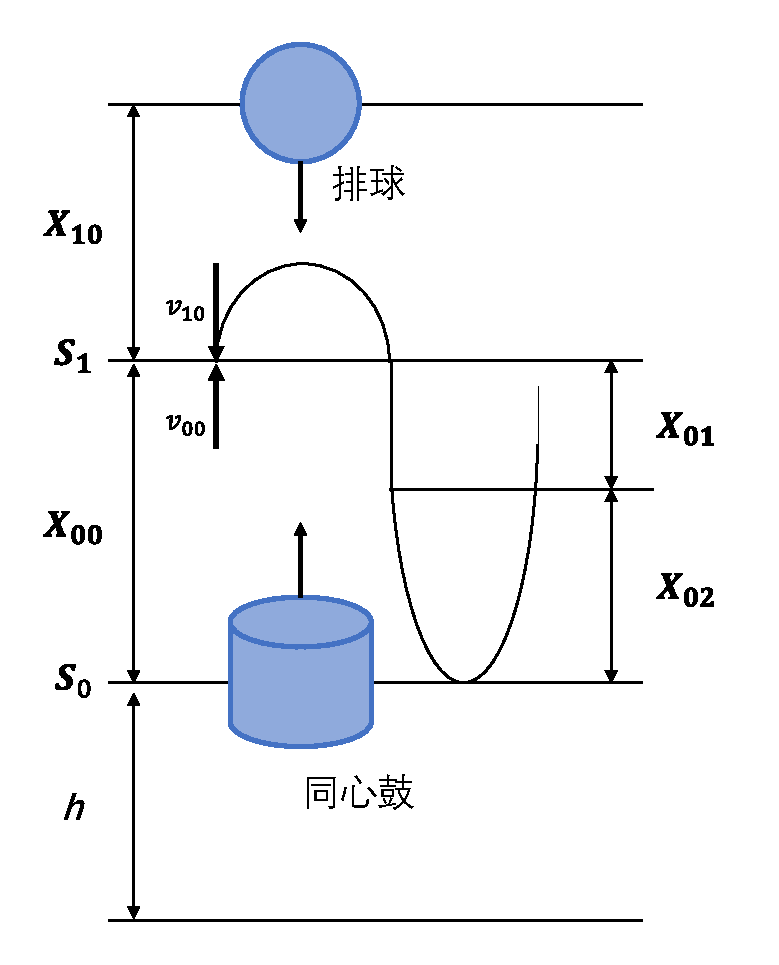
\includegraphics[width=0.8\textwidth]{img/question1.pdf}
\caption{问题一运动过程示意图(未考虑尺寸比例)}\label{fig-buoy}
\end{figure}

\subsection{问题2分析}
题二是一个旋转运动过程研究问题,首先通过空间分析,找出旋转角度之间的关系,然后建立转动模型。分析步骤如下:
\begin{enumerate}
\item 任意选取鼓面上两条半径$AD$,$AH$,长度为$r$,记它们之间夹角为$\gamma$,如图(\ref{figcircle})所示。
\begin{figure}[H]
  \begin{minipage}[t]{0.5\linewidth}
    \centering
    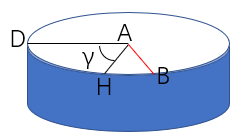
\includegraphics[width=0.8\textwidth]{img/circle.png}
    \caption{鼓面倾斜示意图(一)}
    \label{figcircle}
  \end{minipage}
   \begin{minipage}[t]{0.5\linewidth}
      \centering
      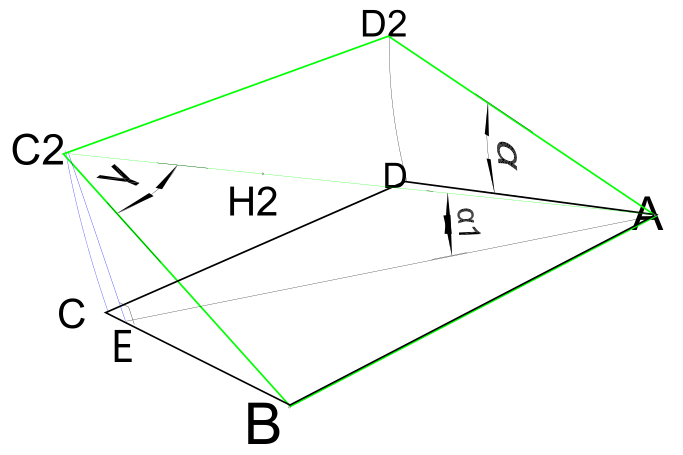
\includegraphics[width=0.8\textwidth]{img/change.png}
      \caption{鼓面倾斜示意图(二)}
      \label{fig:change}
    \end{minipage}
\end{figure}

\quad \quad
假设鼓面沿着与半径$AD$垂直方向的线$AB$为旋转轴倾斜,鼓平面从平面$ABCD$转到了平面$ABC_2D_2$(将两平面均看成长方形分析),旋转角为$\alpha$,如图(\ref{fig:change})所示。$AC$为$AH$所在半径的延长线,则$AC$与$CB$之间夹角为$\gamma$,$AC_2$与$C_2B$之间夹角为$\gamma$。点$E$为点$C_2$在平面$ABCD$的投影,即$C_2E$垂直于$CB$,角$\alpha_1$为倾斜后直线$AC_2$与原平面所夹角。则有:\\
\begin{displaymath}
AC_2=\frac{C_2B}{cos\gamma}
\end{displaymath}
\begin{displaymath}
C_2E=C_2Bsin\alpha
\end{displaymath}
\begin{displaymath}
C_2E=AC_2sin\alpha_1
\end{displaymath}
由以上三式可得出$\alpha_1$与$\alpha$、$\gamma$之间关系为:
\begin{equation}
sin\alpha_1=sin\alpha cos\gamma
\end{equation}

\item 当鼓身上某一绳子的固定端与圆心的连线倾斜了$\alpha$角时,我们记该条绳角度倾斜了$\theta$角,如下图(\ref{fig:angel})所示。因为$\alpha$与$\theta$很小,所以我们近似可得:

\begin{displaymath}
l\theta=r\alpha
\end{displaymath}
不失一般性,我们可推广得到:
\begin{equation}
l\theta_i=r\alpha_i
\end{equation}
\begin{figure}[H]
\centering
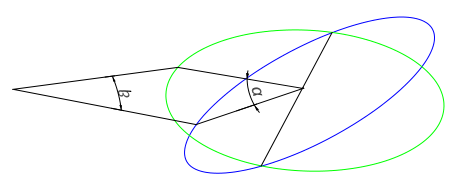
\includegraphics[width=0.5\textwidth]{img/angel.png}
\caption{绳子改变角度示意图}\label{fig:angel}
\end{figure}

\item 由于鼓是一个旋转対称体,所以可将八个固定点分成四组,每两个对称固定点为一组。我们首先考察其中一个固定端。在鼓面为水平时,绳子与水平方向夹角为$\varphi$,当鼓面倾斜了$\alpha$角时,绳子与水平方向角度改变$\theta_1$,则该固定点处绳子与水平方向夹角变为$(\varphi-\theta_1)$,绳子所施加力$F_1$的作用点在平面$AC_2E$上点$H_2$的下方某处,我们可将力分解为竖直方向和沿$AC$方向的力。竖直方向力的大小为$F_1sin(\varphi-\theta_1)$,与直线$AB$距离为$rcos\gamma cos\alpha$;沿$AC$方向力的大小为$F_1cos(\varphi-\theta_1)$,再将其分解为与$AB$直线和与$AD$直线平行的两个力。$F_{AD}$大小为$F_1cos(\varphi-\theta_1)sin\eta$,与直线$AB$距离为$rsin\alpha_1$;因为$F_{AB}$与$AB$平行,所以在鼓倾斜时对力矩不会产生影响;而关于该固定点关于圆心中心对称处的另一固定端处,绳子与竖直方向夹角变为$(\varphi+\theta_1)$,设该处力的大小为$F_2$,所能产生影响的两分解力大小分别为$F_2sin(\varphi+\theta_1)$,$F_2cos(\varphi+\theta_1)sin\eta$,与直线$AB$距离分别为$rcos\gamma cos\alpha$,$rsin\alpha_1$,建立出转动方程。 结合每组的转动方程,可得到关于鼓的转动模型。
\begin{figure}[H]
\centering
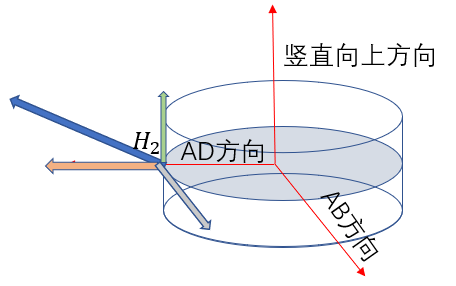
\includegraphics[width=0.8\textwidth]{img/fight.png}
\caption{双面鼓受力示意图}\label{fig:fight}
\end{figure}
\item 分析题目给定数据,选取旋转主轴:某一时刻的旋转主轴方向,即为与此时刻合力方向垂直的鼓面直径所在方向。如图 (\ref{figmain})所示。在某时刻鼓上受到八个力的作用,根据牛顿第一定律,我们可对这八个力进行抵消,$F_1$和$F_2$为抵消后残余的力,$F$为两残余力的合力,它在平面$P$内,则此时的旋转主轴方向就为与平面$P$垂直的$ab$直径所在方向。

\begin{figure}[H]
\centering
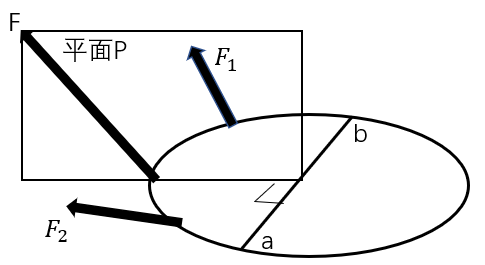
\includegraphics[width=0.8\textwidth]{img/main.png}
\caption{旋转主轴示意图}\label{figmain}
\end{figure}

\item 对序号$1$到序号$9$给定的序号进行分析,我们发现$9$种情况可分为两种类型:对于序号$1$到序号$7$,以及序号$9$,旋转主轴只有一个,旋转主轴可由上述方法得到。而序号$8$在$-0.1s$和$0s$分别有两条不同的旋转主轴。我们首先通过MATLAB对另外八题的鼓面倾角求解,发现在同一时刻由于几位队员多施加了$10N$的力而引起的鼓面倾角变化,相对于队员由于施力时机提早了$0.1$而引起的鼓面倾角变化来说,可以忽略不计,所以我们仍可认为序号$8$的旋转主轴方向始终为$-0.1s$的旋转主轴方向。
\end{enumerate}

\subsection{问题3分析}
通过查阅治疗,人的反应时间为$0.2s$。根据问题二所给数据,结合现实情况,我们将模型分为三种类型讨论,通过MATLAB进行模拟分析。其中,$F$、$F_1$、$F_2$关系式为:$F_1+F_2=2F$,$t_1$、$t_2$、$t_3$关系式为:$t_3-t_2=t_1$。
\begin{itemize}
\item \textbf{类型一} \quad $n$位队员发力大小相同,一位队员提早发力$t_1$。针对此种情况,我们给出两种解决方案:方案一该队员在$0.2s$后意识到自己早发力,于是第$t_2$到第$t_3$期间选择不发力;方案二,对面队员在$0.2s$后意识到队友的错误,于是选择在第$t_2$到第$t_3$期间增大自己的发力大小来弥补错误。
\item \textbf{类型二} \quad $n$位队员同时在第$0s$发力$F_1$,一位队员由于未掌控力度,发力大小为$F$。给出解决方案:该队员在$0.2s$后意识到自己的错误,选择在第$0.2s$到第$0.4s$减少自己的发力,大小为$F_2$。
\item \textbf{类型三} \quad $(n-1)$位队员在第$0s$同时发力$F$,一位队员早发力$t_1$,且发力力度为$F_1$。给出解方案:该队员在发力$0.2s$后将自己的施力力度变为$F_2$,同时其对面队员意识到队友错误增大自己的施力力度。

\end{itemize}
\subsection{问题4分析}
结合问题$(1)$、$(2)$、$(3)$三题的分析解答过程,综合对问题四进行分析。
\begin{enumerate}
\item 我们首先进行运动过程分析。因为鼓对排球的作用力始终是垂直鼓面向上的,所以当排球反弹时相对竖直方向产生$1^{\circ}$倾斜角,说明鼓与排球碰撞时的运动方向夹$0.5^{\circ}$角,则鼓相对水平面的倾斜角度为$0.5^{\circ}$,我们记此时倾角为$-0.5^{\circ}$。所以若想要在下一次碰撞时将排球调整为竖直状态弹跳,则应该使排球倾斜方向变为$+0.5^{\circ}$。如图(\ref{fig:exercise})所示。
\item 对排球在空中的运动进行分析,可计算得到两次碰撞的间隔时间。通过问题一的分析,我们知道在此次碰撞后到下一次碰撞前,鼓经历自由落体运动,减速下降,以及加速上升三个阶段。在此题中为简化问题,我们做如下假设:
\begin{enumerate}
\item 因为我们无需考虑排球上升高度,所以可假定减速加速两过程所施加的力是一样的。那么在变速运动阶段,鼓由于受力不均而发生倾斜,由于我们认为在此过程中每个人施力情况不变,那么鼓做匀速翻转。我们想要使鼓的倾斜角度从$-0.5^{\circ}$变为$+0.5^{\circ}$,所以当鼓水平时刚好为变速运动中间时刻。
\item 由于碰撞时鼓的速度不可知,我们可假定碰撞后鼓立即以速度$0m/s$自由落体。通过对排球运动时间分析,可计算得到队员作用力的时机、作用时间。
\item 假定鼓面初始位置较绳子水平时仍下降$11cm$。
\end{enumerate}

\begin{figure}[H]
\centering
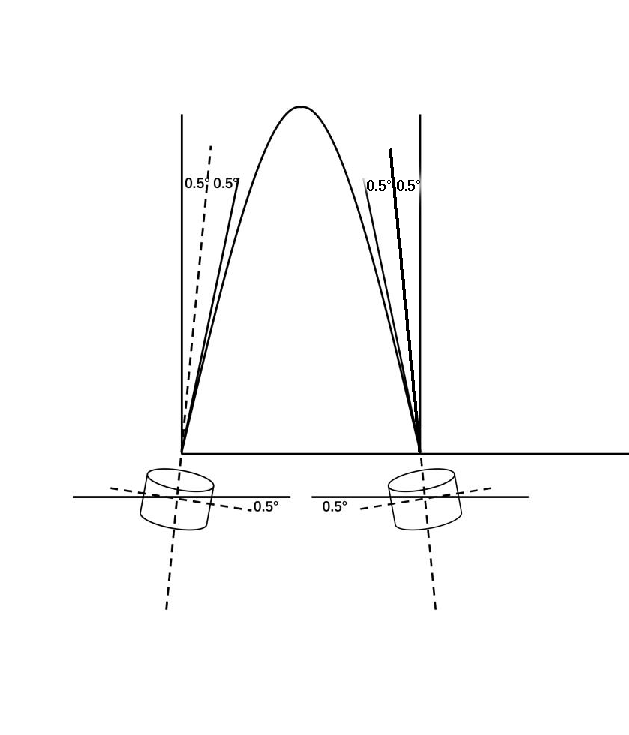
\includegraphics[width=0.8\textwidth]{img/exercise.pdf}
\caption{旋转主轴示意图}\label{fig:exercise}
\end{figure}
\item 开始时,我们假设$10$位队员每人施加力的时机和力度都相同,通过分析计算可发现在这种情况下,第二次碰撞时鼓的倾斜角度并不为$0.5^{\circ}$。然后在保持原有的合力大小不变的基础上,逐渐增加几位队员施加力,而减少其余队员施加力,利用MATLAB对该过程进行逐步模拟分析,直至找出最终使鼓倾斜角度为$0.5^{\circ}$时,每位队员施加力的情况。

\item 模拟在现实情况下,由于队员的用力时机和大小都无法完全遵从理想值,我们在理想值的基础上,对施力时间和大小上都加上了一个正态分布的扰动,并且多次进行实验模拟随机情况下纪律扰动带来的角度变化(如图)。由图可以明显看出,绝大部分倾斜角度的振幅都大于0.5°,而现实情况下补救措施中发力的误差也不可避免,极大概率也会带来超过0.5°的扰动,这说明鼓面0.5°的倾斜在现实情况下是不可避免的。
\begin{figure}[H]
\centering
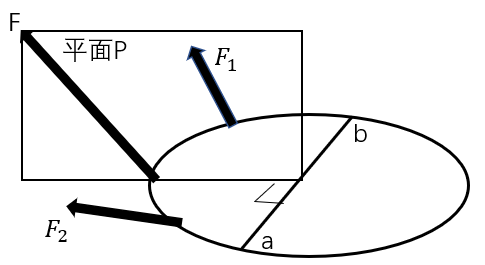
\includegraphics[width=0.8\textwidth]{img/main.png}
\caption{旋转主轴示意图}\label{figmain}
\end{figure}

\end{enumerate}

\subsection{问题1的解答}
\begin{enumerate}
\item \textbf{绳长计算}\\
我们假设团队队员共有$n$人,每人之间的距离为最小距离$60cm$。队员牵拉绳子的水平投影线的延长线交于绳子固定端所在圆的圆心$A$,则该圆心与两队员队员所站位置可构成水平的等腰三角形,三角形顶角为$\frac{360^{\circ}}{n}$,三角形底角角度为($90^{\circ}-\frac{180^{\circ}}{n}$),如下图所示:
\begin{figure}[H]
\centering
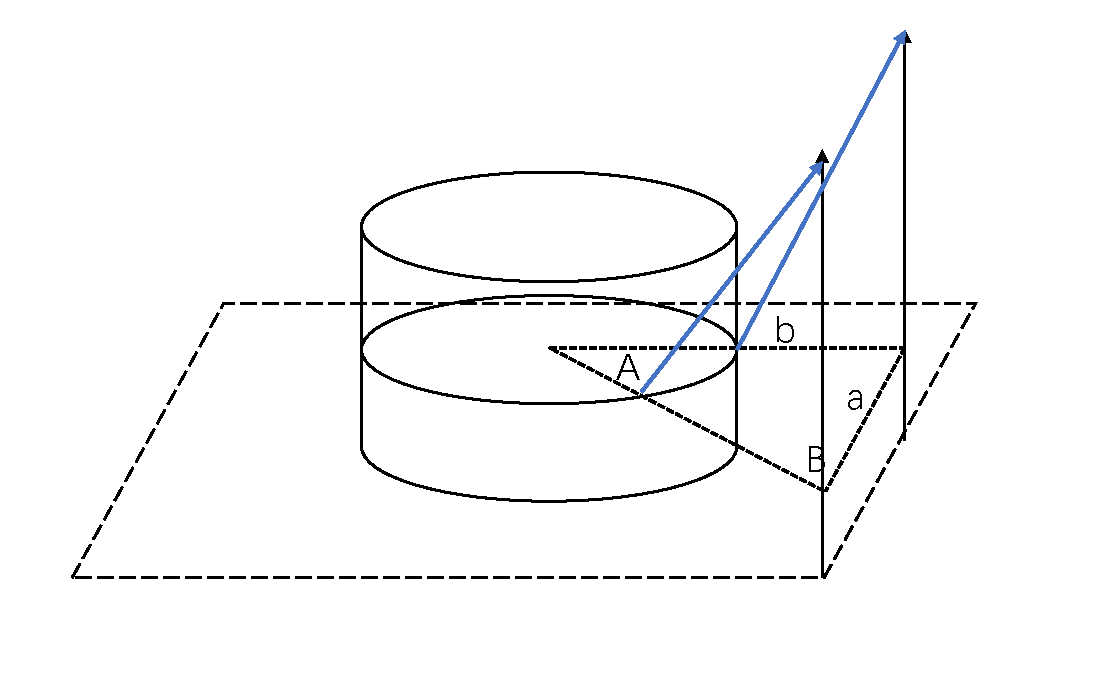
\includegraphics[width=0.8\textwidth]{img/string.pdf}
\caption{绳长计算示意图}
\end{figure}
由正弦定理可得:
\begin{displaymath}
\frac{a}{sinA}=\frac{b}{sinB}
\end{displaymath}
即:
\begin{displaymath}
\frac{0.6}{sin({\frac{360^{\circ}}{n}})}=\frac{b}{sin({90^{\circ}-\frac{180^{\circ}}{n}})}
\end{displaymath}
解得$b$的长度为:
\begin{displaymath}
b=\frac{0.3}{sin( \frac{180^{\circ}}{n})}
\end{displaymath}
又因为绳子与水平方向夹角为$\varphi$,所以绳子长度可以表示为:
\begin{displaymath}
l=\frac{b-r}{cos\varphi}=\frac{\frac{0.3}{sin(\frac{180^{\circ}}{n})}-r}{cos\varphi}
\end{displaymath}
在此题中,假设$n=8$人。
所以有:
\begin{equation}
l=\frac{0.3\sqrt{2}-0.2}{cos\varphi}
\end{equation}
在最佳策略下每人施加力度应尽可能小,那么应尽量减小绳子与竖直方向夹角,所以此时设定$h=0$,即$s_0$在水平地面上。手的作用高度与绳子在鼓身固定端的高度差为$1.2-(\frac{0.22}{2})=1.09m$。
\begin{equation}
sin\varphi=\frac{1.09}{l}
\end{equation}
结合式子$(3)$、$(4)$,计算得到绳子长度为$l=1.16661m$。
\item \textbf{运动计算}\\
在最佳协作策略下,每位队员都想要使自己施加的力尽可能小,持续时间尽可能短。这样我们可以假设排球所能到达的最高高度恰好为$40cm$。
在第一阶段中,排球从最高处自由落到碰撞位置的时间与鼓从$s_0$上升到碰撞位置的时间相等,可列公式:
\begin{equation}
\frac{v_{00}}{a_1}=\frac{v_{10}}{g}
\end{equation}
且有$x_{00}+x_{10}=0.4$,即:
\begin{equation}
\frac{v^2_{10}}{2g}+\frac{v^2_{00}}{2a_1}=0.4
\end{equation}
在二、三、阶段中,排球从碰撞位置回到最高点的时间与鼓从碰撞位置回到$s_0$的时间相等,可列公式:
\begin{equation}
\frac{v_{11}}{g}=\frac{v_{02}+v_{01}}{g}+\frac{v_{02}}{a_2}
\end{equation}
且有$x_{10}+x_{01}+x_{02}=0.4$,则:
\begin{equation}
\frac{v^2_{11}}{2g}+\frac{(v^2_{02}-v^2_{01})}{g}+\frac{v^2_{02}}{a_2}=0.4
\end{equation}
排球做自由落体运动,在同一高度时速度大小相同,则有:
\begin{equation}
v_{11}=v_{10}
\end{equation}
碰撞时,由动量守恒可列公式:
\begin{equation}
m_0v_{00}-m_1v_{11}=m_0v_{01}+m_1v_{11}
\end{equation}
通过查阅相关资料,我们设定碰撞恢复系数大小为$0.74$,所列公式为:
\begin{equation}
e=\frac{v_{11}-v_{01}}{v_{00}+v_{11}}
\end{equation}


\item \textbf{计算求解}\\
结合方程$(5)$到方程$(11)$,利用MATLAB求解,得到结果:
$$v_{00}=0.593537m/s$$
$$v_{01}=0.2157m/s$$
$$v_{02}=0.669324m/s$$
$$v_{11}=v_{10}=2.51891m/s$$
$$F_1=5.83214N$$
$$F_2=6.65350N$$
\quad \quad
算得第一阶段时间为$0.257032s$,第二阶段时间为$0.0903086s$,第三阶段时间为$0.166724s$。
所以最佳策略为当球从最高处下落时,每位队员施加$5.83214N$的力,持续时间为$0.257032s$,与排球碰撞,使排球弹起,最高点仍能回到$40cm$,碰撞$0.0903086s$后,每位队员施加$6.65350N$大小的力,持续$0.166724s$,使鼓减速回到$s_0$。

\end{enumerate}

\subsection{问题2的解答}
在问题二中,$sin\varphi$计算结果为$0.0647$。
\begin{figure}[H]
\centering
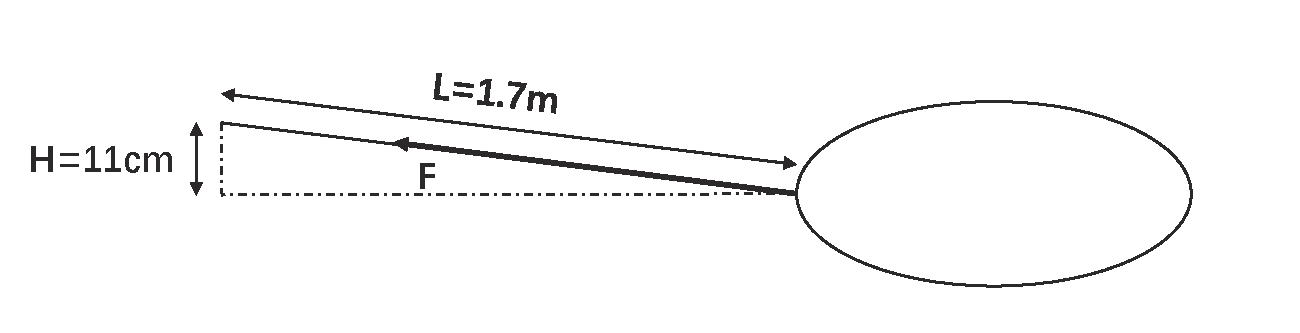
\includegraphics[width=0.8\textwidth]{img/string1.pdf}
\caption{绳长计算示意图}
\end{figure}
通过对问题二的分析,我们可将八个固定端分成四组,每两个相对称的固定端为一组,某一固定端转动方程为:
\begin{equation}
J\beta_{1i}= F_{1i}sin(\varphi-\theta_i)rcos\gamma cos\alpha- F_{1i}cos(\varphi-\theta_i)rsin\eta sin\varphi_i
\end{equation}
其对称处转动方程为:
\begin{equation}
J \beta_{2i}= F_{2i}sin(\varphi+\theta_i)rcos\gamma cos\alpha+F_{2i}cos(\varphi+\theta_i)rsin\eta sin\varphi_i
\end{equation}
综合所有固定端,得到鼓的转动方程如下:
\begin{equation}
J \beta=\sum_{i=1}^4 (J\beta_{i1}-J\beta_{i2})
\end{equation}
\quad \quad
结合公式$(1)$、$(2)$、$(12)$、$(13)$、$(14)$, 利用MATLAB进行小步长求解,得到结果如表\ref{table-sym}所示。
由于初始时,每位队员施加力的力度和时机不同,我们假定在开始时由于施力不均而造成鼓面旋转的方向为正方向。
\begin{table}[H]
\centering
\caption{鼓面倾斜角度结果}\label{table-sym}
\begin{tabular}{|c|c|c|c|c|c|c|c|c|c|c|}
\hline
序号 & 用力参数 & 1    & 2    & 3  & 4    & 5    & 6  & 7  & 8    & 鼓面倾角(度) \\
\hline
1  & 发力时机 & 0    & 0    & 0  & 0    & 0    & 0  & 0  & 0    &   $0.198926^{\circ}$ \\
   & 用力大小 & 90   & 80   & 80 & 80   & 80   & 80 & 80 & 80   &       \\
\hline
2  & 发力时机 & 0    & 0    & 0  & 0    & 0    & 0  & 0  & 0    &    $0.361033^{\circ}$ \\
   & 用力大小 & 90   & 90   & 80 & 80   & 80   & 80 & 80 & 80   &         \\
\hline
3  & 发力时机 & 0    & 0    & 0  & 0    & 0    & 0  & 0  & 0    &    $0.154996^{\circ}$ \\
   & 用力大小 & 90   & 80   & 80 & 90   & 80   & 80 & 80 & 80   &         \\
\hline
4  & 发力时机 & -0.1 & 0    & 0  & 0    & 0    & 0  & 0  & 0    &    $-2.33284^{\circ}$ \\
   & 用力大小 & 80   & 80   & 80 & 80   & 80   & 80 & 80 & 80   &         \\
\hline
5  & 发力时机 & -0.1 & -0.1 & 0  & 0    & 0    & 0  & 0  & 0    &    $-3.90435^{\circ}$ \\
   & 用力大小 & 80   & 80   & 80 & 80   & 80   & 80 & 80 & 80   &         \\
\hline
6  & 发力时机 & -0.1 & 0    & 0  & -0.1 & 0    & 0  & 0  & 0    &    $-1.9634^{\circ}$  \\
   & 用力大小 & 80   & 80   & 80 & 80   & 80   & 80 & 80 & 80   &         \\
\hline
7  & 发力时机 & -0.1 & 0    & 0  & 0    & 0    & 0  & 0  & 0    &    $-2.49741^{\circ}$ \\
   & 用力大小 & 90   & 80   & 80 & 80   & 80   & 80 & 80 & 80   &         \\
\hline
8  & 发力时机 & 0    & -0.1 & 0  & 0    & -0.1 & 0  & 0  & 0    &   $ -1.95983^{\circ}$ \\
   & 用力大小 & 90   & 80   & 80 & 90   & 80   & 80 & 80 & 80   &         \\
\hline
9  & 发力时机 & 0    & 0    & 0  & 0    & -0.1 & 0  & 0  & -0.1 &   $ -2.14966^{\circ}$ \\
   & 用力大小 & 90   & 80   & 80 & 90   & 80   & 80 & 80 & 80   &        \\
\hline
\end{tabular}
\end{table}
\subsection{问题3解答}
针对类型一、二、三给出的策略,利用MATLAB模拟分析,有如下结果(假定人数$n=8$):
\begin{itemize}
\item \textbf{类型一策略一}\\
对于类型一,所有队员发力大小相同(令$F_1=80N$),但某一队员提早$t_1$发力。给出策略:该队员在反应了$0.2s$后意识到自己的错误,于是选择在$0.2s$后持续$t_1$不发力。假定该队员提早发力$0.1s$,于是在第$0.1s$到第$0.3s$期间选择不发力。通过MATLAB模拟分析,给出了在有策略(不发力)和无策略(保持原有力)两种情况下,鼓面倾斜角度变化,如图(\ref{figtype1})所示。发现两种情况下鼓面倾斜角度无明显区别,该策略无效。
\begin{figure}[H]
\centering
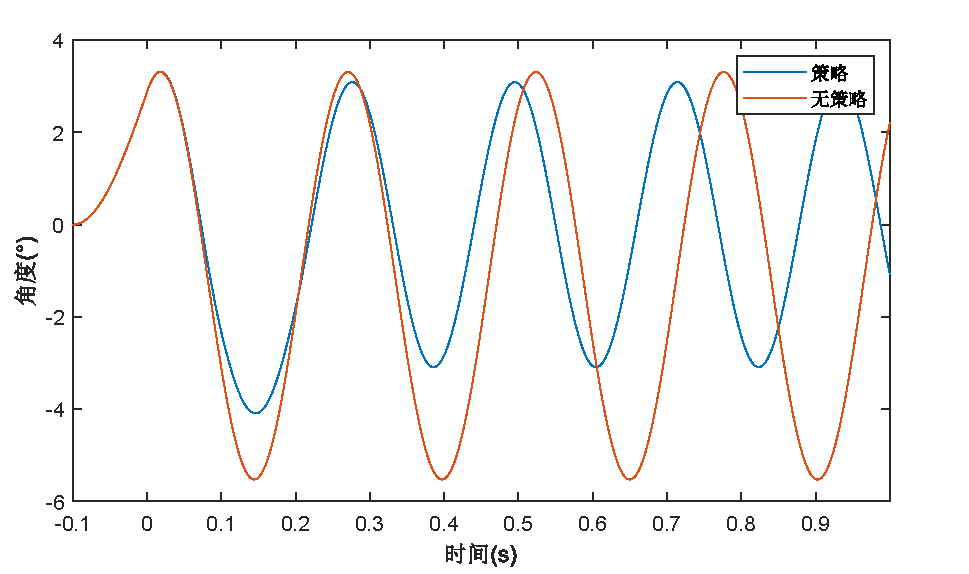
\includegraphics[width=0.8\textwidth]{img/type1.pdf}
\caption{类型一策略一结果图}
\label{figtype1}
\end{figure}
\item \textbf{类型一策略二}\\
对于类型一,所有队员发力大小相同(令$F_1=80N$),但某一队员提早发力。给出策略:对面队员在反应了$0.2s$后,通过改变自己施力大小弥补队友错误。我们假定一队员提早发力$0.1s$,那么对面队友在第$0.1s$到第$o.2s$期间改变自己的用力。利用MATLAB对未实施策略、对面队友实施力改变为$160N$、$240N$、$320N$、$400N$五种情况进行分析,得到如图(\ref{figtype2})所示结果。发现当对面队友逐渐增加自己的实施力,鼓面倾斜程度波动范围逐渐变小,$400N$时我们可认为鼓面维持在水平。
\begin{figure}[H]
\centering
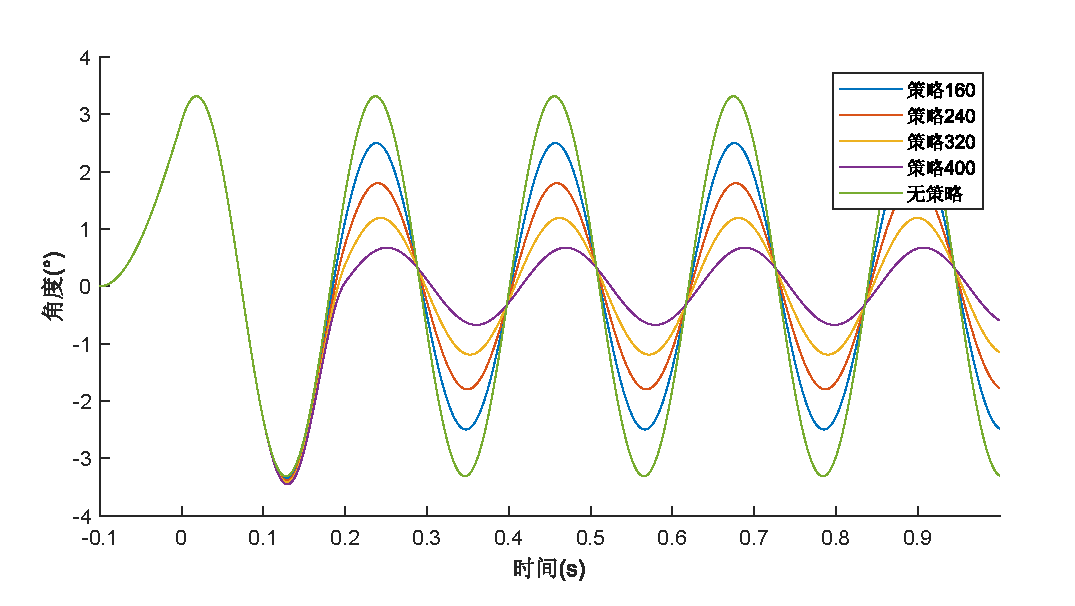
\includegraphics[width=0.8\textwidth]{img/type2.pdf}
\caption{类型一策略二结果图}
\label{figtype2}
\end{figure}


\item \textbf{类型二策略}\\
对于类型二,所有队员同时发力,但某一队员未能掌控施力力度情况。给出策略:该队员在反应了$0.2s$后,改变自己的施力力度。令$F_1=90N$,$F=80N$带入分析,通过MATLAB对实施策略和未实施策略两种情况进行分析,得到如图(\ref{figtype3})所示结果。发现当未实施策略时,鼓面倾斜角度会以$0.1^{\circ}$的均值,在$0^{\circ}$到$0.2^{\circ}$之间进行大幅度波动。而当实施了策略时,鼓面倾斜角度在$0^{\circ}$附近进行小幅波动,说明可以使鼓面维持水平的效果更好,该策略有效。

\begin{figure}[H]
\centering
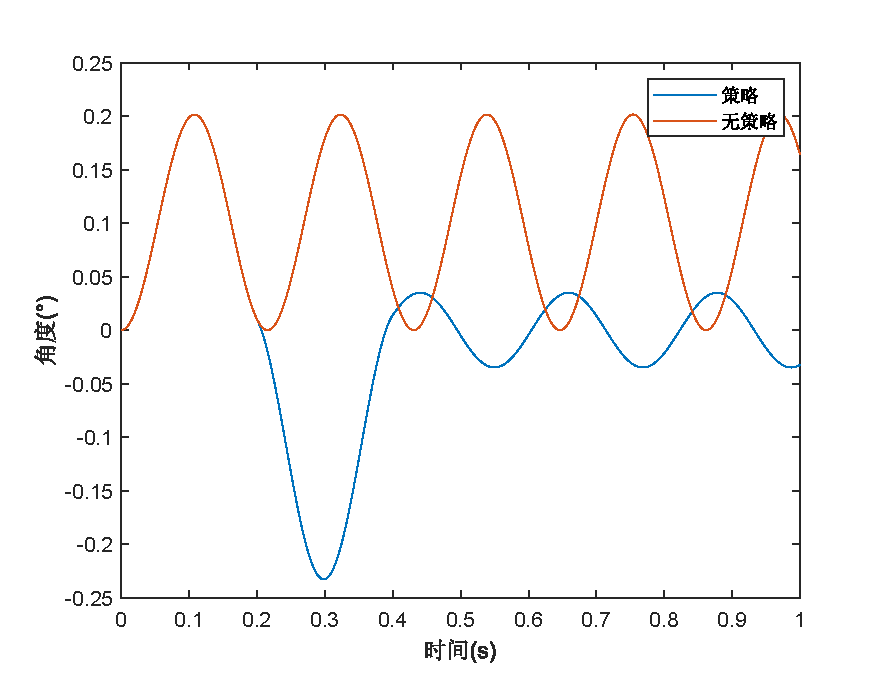
\includegraphics[width=0.8\textwidth]{img/type3.pdf}
\caption{类型二策略结果图}
\label{figtype3}
\end{figure}
\item \textbf{类型三策略}\\
对于类型三,$7$位队员同时发力$F$,但某一队员未能掌控发力时机及力度。给出策略:该队员在反应了$0.2s$后,改变自己的施力力度,同时其对面队友也改变自己的施力力度来弥补队友的错误。假定具体数据,一队员提早发力$0.1s$,且施力力度为$90N$。在第$0.1s$意识到错误,于是第$0.1s$到第$0.3s$将自己的施力改变为$70N$。同时在第$0.1s$到第$0.2s$对面队员改变自己的施力力度(有类型一策略二可知该方法有效)。通过MATLAB对实施策略和未实施策略两种情况进行分析,同时将有策略情况分为对面队友分别实施$160N$、$240N$、$320N$、$400N$五种情况,得到如图(\ref{figtype4})所示结果。发现在实施了策略后,鼓面倾斜角度有明显减小,且对面队员施力大小越大效果越明显,该策略有效。
\begin{figure}[H]
\centering
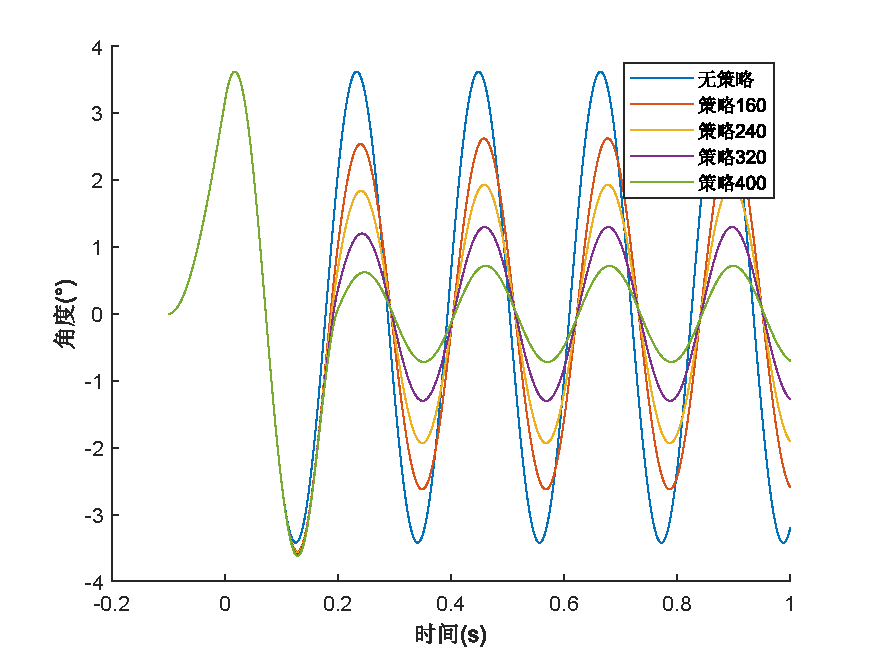
\includegraphics[width=0.8\textwidth]{img/type4.pdf}
\caption{类型三策略结果图}
\label{figtype4}
\end{figure}



\end{itemize}
\subsection{问题4解答}
\begin{enumerate}
\item \textbf{排球运动分析}\\
排球在空中做加速度恒为$g=9.8m/s$的运动,且能达到的最高高度为$h=60cm$,所以根据运动方程:
\begin{displaymath}
\frac{1}{2}gt^2=h
\end{displaymath}
得到在空中运动时间为$2t=0.670s$,即两次碰撞间隔时间为$0.670s$。
\item\textbf{鼓运动计算}\\
我们假设鼓自由落体时间为$t_1$,变速运动时间为$t_2$,加速度为$a$,由于自由落体与变速运动两阶段位移相等。所以有:
\begin{equation}
\frac{1}{2}gt^2=-gt_1t_2+\frac{1}{2}at_2^2
\end{equation}
两次碰撞间隔,鼓运动时间与排球运动时间相等,可得等式:
\begin{equation}
t_1+t_2=2t
\end{equation}
我们仍假设鼓面初始位置较绳子水平时下降 $11cm$。
\begin{equation}
a=\frac{Fsin\varphi-mg}{m}
\end{equation}
综合式子$(15)$到$(17)$,可计算得到$t_1$为$0.1804s$,$t_2$为$0.5193s$。
\item \textbf{排球受力分析}\\
现在,我们对鼓的旋转主轴进行分析。现有十位队员参与比赛,我们分别标记为$1,2,3,\dots,10$,那么每两位队员所拉绳子的固定端与圆心的夹角为$36^{\circ}$。根据题意,排球倾斜方向在水平面的投影指向某两位队员之间,且与这两位队员的夹角之比为$1:2$。我们假设排球倾斜方向的投影落在队员$1$与队员$2$之间,与队员$1$的夹角为$24^{\circ}$,与队员$2$的夹角为$12^{\circ}$。图(\ref{fig:ball})为鼓面俯视图,$oc$为排球倾斜方向投影,那么鼓的旋转主轴方向应与$oc$垂直,可找出过圆心的直线$ab$为旋转主轴方向。而由于离旋转主轴越远,对旋转的影响越大,所以我们增加队员$2$、$7$施加的力,减少其余队员的施加力,逐步分析直至第二次碰转角度为$0.5^{\circ}$。
\begin{figure}[H]
\centering
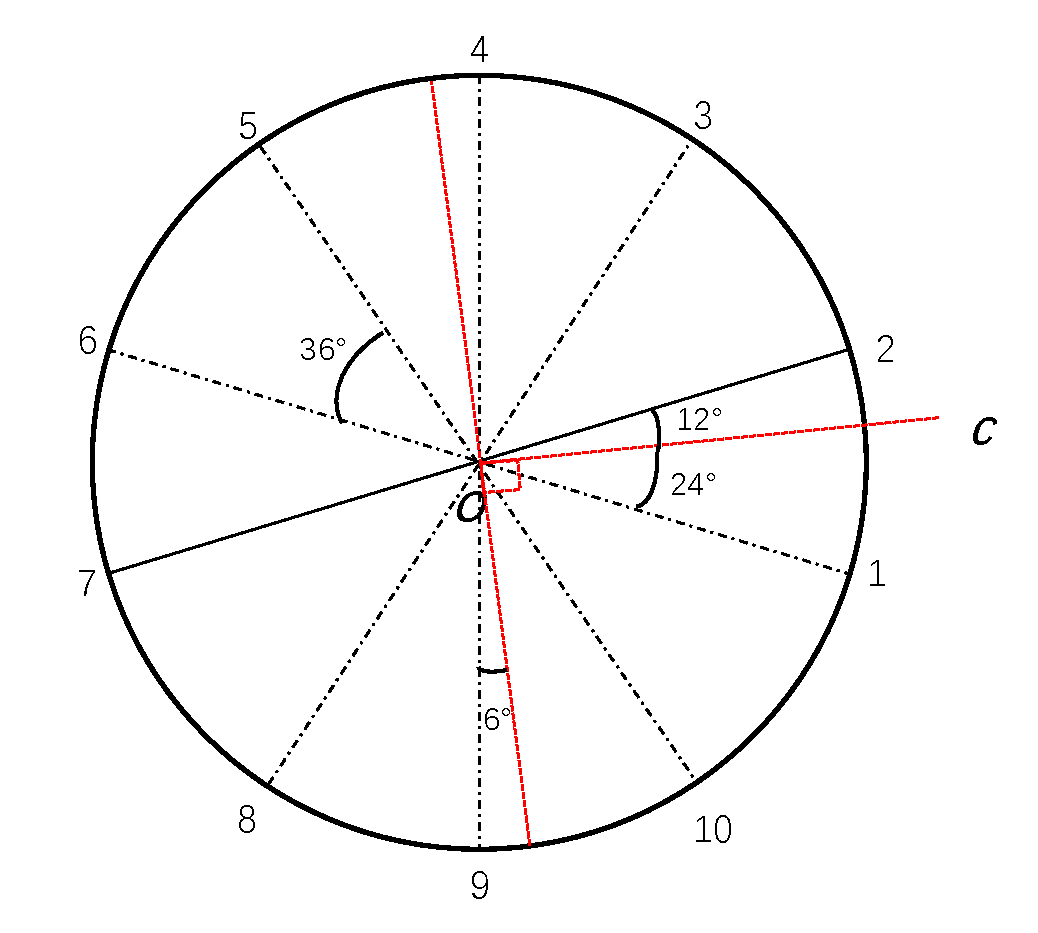
\includegraphics[width=0.8\textwidth]{img/ball.pdf}
\caption{鼓面俯视图}\label{fig:ball}
\end{figure}

\item \textbf{扰动情况分析}
\begin{itemize}

\item 为了保证鼓面不围绕其他转轴发生转动,并且使用最小的力达到转动鼓面的效果,将图(\ref{fig:ball})中$2$、$7$两对称点的力数值等比例增大,为了尽可能保证鼓面在竖直方向上的位移不受影响,假设所有队员用力的数值和为800N。于是,可得下式:

然后对不同的F进行受力分析得到角度方程如下:

运用计算机进行模拟可以得到不同F下的倾斜角度,进行小步长搜索得到目标可行解如下。

\item 现在考虑现实情况下的调整措施的可行性,考虑到现实情况下队员的发力时机和大小无法完全遵从理想值,故在发力时机和大小的理想值基础上叫上正态分布的扰动,由$3\sigma$原则确定相应的$\sigma$值,得到发力时机和发力大小表达式如下:

根据上面的每一组发力时机和大小,运用计算机模拟鼓面的倾斜角度变化,得到多组实验图像如下:

由图可知,现实情况下队员用力误差产生鼓面倾斜的角度大多数情况下大于0.5°,鼓面倾斜的调整策略产生的误差大于0.5°,所以在现实情况下没有意义。
\end{itemize}

\end{enumerate}

\section{模型总结}

\subsection{模型优点}
\begin{enumerate}
\item 在问题一中,我们在满足题设条件的情况下,提出了一个在理想条件下适用的物理模型,使得每位队员施加力的时间及力度可达到最小,不费精力。
\item 对于问题二的模型,我们运用空间几何分析,考虑了由于鼓面的倾斜导致各个绳子固定点的高度不同,进而导致绳子上作用力与转轴之间的角度变化,导致产生的力矩发生了变化,提升了分析的精度和准确性。
\item 对于问题三,我们对于队员产生误差的情况进行了分类,并且根据各个情况的具体情况运用对称性原理,提出了合理的调整策略,并且对比了使用策略与否的鼓面倾斜情况验证了策略的可行性。
\item 在问题四中,我们利用计算机对所有队员的力度进行小步长的搜索,来获取队员力度的可行解。并且通过模拟显示在现实生活中正态分布的的误差,对鼓的倾斜角度变化情况进行模拟,结合结论说明了一定程度的倾斜在现实情况下是难以避免的。
\end{enumerate}

\subsection{模型缺点}
\begin{enumerate}
\item 问题一模型:忽略了由于鼓面的高度变化带来的绳子作用力方向的变化引起的角加速度的变化。
\item 问题二模型:在题目第八组的分析中,我们忽略了与原转动方向相异的轻微转动带来的扰动在垂直转轴方向上产生的转动分量,导致结果相较于真实情况有一定的误差。
\item 问题三模型:未能考虑现实情况中多个成员发力时机与力度产生变化带来的误差的调整策略。
\item 问题四模型:未能考虑到高度变化带来的所有绳子作用力方向与竖直方向间的角度变化。
\end{enumerate}


\bibliographystyle{plain}
\bibliography{ref}
\begin{thebibliography}{99}
\bibitem{1}
\bibitem{2}
\end{thebibliography}

\newpage
\appendix
\textbf{附录}
\section{问题一求解代码}
\begin{lstlisting}[language=matlab]
clc
clear
syms n h step F1 F2 v00 v11 v01 v02 h11 n
% e 为鼓与球碰撞的恢复系数。
e = 0.74; m0 = 3.6; m1 = 0.27; g = 9.8; d = 0.4; r = d / 2;
% h_min 为球颠起后需要距离鼓的最小距离40cm。
h_min = 0.4;
n = input('Please input the number of students:');
h = input('Please input the height of the hand:');
% h0 为鼓距离地面的距离。
h0 = 0.11;
% alpha 人与人之间的角度。
alpha = 360/n;
% 绳长
lx = sqrt(0.6^2 / (2 * (1 - cos(alpha)))) - r;
ly = h - h0;
l = sqrt(lx^2 + ly^2);

phi = asin(ly / l);
% a1 为鼓上升时候的加速度, a2 为鼓下降第二段的加速度
a1 = (n * F1 * sin(phi) - m0 * g)/m0;
a2 = (n * F2 * sin(phi) - m0 * g)/m0;

equ1 = m0 * v00 - m1 * v11 == m0 * v01 + m1 * v11;
equ2 = (v11 - v01) / (v00 + v11) == e;
equ3 = a1 * v11 == g * v00;
equ4 = v11/g == (v02 + v01)/g + v02/a2;
equ5 = v11^2/g + v00^2/a1 == 0.8;
equ6 = v11^2/g + (v02^2 - v01^2)/g + v02^2/a2 == 0.8;
equ = [equ1, equ2, equ3, equ4, equ5, equ6];
[F1, F2, v00, v01, v02, v11] = solve(equ, [F1, F2, v00, v01, v02, v11]);
fprintf('施加的力F1为:%.5f\n施加的力F2为:%.5f\n绳子长度为:%g\n',F1(2), F2(2), l);
fprintf('v00 = %g\nv01 = %g\nv02 = %g\nv11 = %g\n', v00(2), v01(2), v02(2), v11(2));
a1 = (n * F1(2) * sin(phi) - m0 * g)/m0;
a2 = (n * F2(2) * sin(phi) - m0 * g)/m0;
t1 = v00(2) / a1;
t2 = (v01(2) + v02(2)) / g;
t3 = v02(2) / a2;
fprintf('上升时间:%g\n下降第一段时间:%g\n下降第二段时间:%g\n', t1, t2, t3);

\end{lstlisting}

\section{问题二代码}
\subsection{子问题一}
\begin{lstlisting}[language=matlab]
clc
clear
d = 0.4; r = d/2; m = 3.6; h = 0.22;
F1 = 90; F2 = 80;
l = 1.7;
phi = asin(0.11/1.7); alpha = 0; omega = 0;
gamma1 = 0; gamma2 = pi / 4;
J = 1/2 * m * r^2 + 1/12 * m * h^2; %圆环的转动惯量。
step = 1000000;
t = 0.1 / step; % 0.1 秒的步长。

for i=1:step
    alpha1 = asin(sin(alpha) * cos(gamma1));
    alpha2 = asin(sin(alpha) * cos(gamma2));
    Eta1 = acos(sin(gamma1) / cos(alpha1));
    Eta2 = acos(sin(gamma2) / cos(alpha2));
    theta1 = alpha1 * r / l;
    theta2 = alpha2 * r / l;
    % 转动方程求此时的角加速度。
    beta = (r * (F1 * (sin(phi - theta1) * cos(alpha) * cos(gamma1) - cos(phi - theta1) * sin(alpha1) * sin(Eta1)) - ...
        F2 * (sin(phi + theta1) * cos(alpha) * cos(gamma1) + cos(phi + theta1) * sin(alpha1) * sin(Eta1))) + ...
        2 * F2 * r * (sin(phi - theta2) * cos(alpha) * cos(gamma2) - cos(phi - theta2) * sin(alpha2) * sin(Eta2) - ...
        sin(phi + theta2) * cos(alpha) * cos(gamma2) - cos(phi + theta2) * sin(alpha2) * sin(Eta2))) / J;
    alpha = alpha + omega * t + 1/2 * beta * t^2;
    omega = omega + beta * t;
end
fprintf('鼓面倾角:%g°\n', rad2deg(alpha));
\end{lstlisting}

\subsection{子问题二}
\begin{lstlisting}[language=matlab]
clc
clear
d = 0.4; r = d/2; m = 3.6; h = 0.22;
F1 = 90; F2 = 80;
l = 1.7;
phi = asin(0.11/1.7); alpha = 0; omega = 0;
gamma1 = pi / 8; gamma2 = 3 * pi / 8;
J = 1/2 * m * r^2 + 1/12 * m * h^2; %圆环的转动惯量。
step = 1000000;
t = 0.1 / step; % 0.1 秒的步长。

for i=1:step
    alpha1 = asin(sin(alpha) * cos(gamma1));
    alpha2 = asin(sin(alpha) * cos(gamma2));
    Eta1 = acos(sin(gamma1) / cos(alpha1));
    Eta2 = acos(sin(gamma2) / cos(alpha2));
    theta1 = alpha1 * r / l;
    theta2 = alpha2 * r / l;
     % 转动方程求此时的角加速度。
    beta = (2 * r * (F1 * (sin(phi - theta1) * cos(alpha) * cos(gamma1) - cos(phi - theta1) * sin(alpha1) * sin(Eta1)) - ...
        F2 * (sin(phi + theta1) * cos(alpha) * cos(gamma1) + cos(phi + theta1) * sin(alpha1) * sin(Eta1))) + ...
        2 * F2 * r * (sin(phi - theta2) * cos(alpha) * cos(gamma2) - cos(phi - theta2) * sin(alpha2) * sin(Eta2) - ...
        sin(phi + theta2) * cos(alpha) * cos(gamma2) - cos(phi + theta2) * sin(alpha2) * sin(Eta2))) / J;
    alpha = alpha + omega * t + 1/2 * beta * t^2;
    omega = omega + beta * t;
end
fprintf('鼓面倾角:%g°\n', rad2deg(alpha));
\end{lstlisting}

\subsection{子问题三}
\begin{lstlisting}[language=matlab]
clc
clear
d = 0.4; r = d/2; m = 3.6; h = 0.22;
F1 = 90; F2 = 80;
l = 1.7;
phi = asin(0.11/1.7); alpha = 0; omega = 0;
gamma2 = pi / 8; gamma1 = 3 * pi / 8;
J = 1/2 * m * r^2 + 1/12 * m * h^2; %圆环的转动惯量。
step = 1000000;
t = 0.1 / step; % 0.1 秒的步长。

for i=1:step
    alpha1 = asin(sin(alpha) * cos(gamma1));
    alpha2 = asin(sin(alpha) * cos(gamma2));
    Eta1 = acos(sin(gamma1) / cos(alpha1));
    Eta2 = acos(sin(gamma2) / cos(alpha2));
    theta1 = alpha1 * r / l;
    theta2 = alpha2 * r / l;
     % 转动方程求此时的角加速度。
    beta = (2 * r * (F1 * (sin(phi - theta1) * cos(alpha) * cos(gamma1) - cos(phi - theta1) * sin(alpha1) * sin(Eta1)) - ...
        F2 * (sin(phi + theta1) * cos(alpha) * cos(gamma1) + cos(phi + theta1) * sin(alpha1) * sin(Eta1))) + ...
        2 * F2 * r * (sin(phi - theta2) * cos(alpha) * cos(gamma2) - cos(phi - theta2) * sin(alpha2) * sin(Eta2) - ...
        sin(phi + theta2) * cos(alpha) * cos(gamma2) - cos(phi + theta2) * sin(alpha2) * sin(Eta2))) / J;
    alpha = alpha + omega * t + 1/2 * beta * t^2;
    omega = omega + beta * t;
end
fprintf('鼓面倾角:%g°\n', rad2deg(alpha));
\end{lstlisting}

\subsection{子问题四}
\begin{lstlisting}[language=matlab]
clc
clear
d = 0.4; r = d/2; m = 3.6; h = 0.22;
F1 = 90; F2 = 80;
l = 1.7;
phi = asin(0.11/1.7); alpha = 0; omega = 0;
gamma1 = 0; gamma2 = pi / 4;
J = 1/2 * m * r^2 + 1/12 * m * h^2; %圆环的转动惯量。
step = 1000000;
t = 0.1 / step; % 0.1 秒的步长。

for i=1:step
    alpha1 = asin(sin(alpha) * cos(gamma1));
    Eta1 = acos(sin(gamma1) / cos(alpha1));
    theta1 = alpha1 * r / l;
     % 转动方程求此时的角加速度。
    beta = r * F2 * (sin(phi - theta1) * cos(alpha) * cos(gamma1) - cos(phi - theta1) * sin(alpha1) * sin(Eta1)) / J;
    alpha = alpha + omega * t + 1/2 * beta * t^2;
    omega = omega + beta * t;
end
fprintf('0.1s前的鼓面倾角:%g°\n', rad2deg(alpha));
for i=1:step
%     if mod(i,10) == 0
%         fprintf('%d\n', i/10);
%     end
    alpha1 = asin(sin(alpha) * cos(gamma1));
    alpha2 = asin(sin(alpha) * cos(gamma2));
    Eta1 = acos(sin(gamma1) / cos(alpha1));
    Eta2 = acos(sin(gamma2) / cos(alpha2));
    theta1 = alpha1 * r / l;
    theta2 = alpha2 * r / l;
     % 转动方程求此时的角加速度。
    beta = (F2 * r * (sin(phi - theta1) * cos(alpha) * cos(gamma1) - cos(phi - theta1) * sin(alpha1) * sin(Eta1) - ...
        sin(phi + theta1) * cos(alpha) * cos(gamma1) - cos(phi + theta1) * sin(alpha1) * sin(Eta1)) + ...
        2 * F2 * r * (sin(phi - theta2) * cos(alpha) * cos(gamma2) - cos(phi - theta2) * sin(alpha2) * sin(Eta2) - ...
        sin(phi + theta2) * cos(alpha) * cos(gamma2) - cos(phi + theta2) * sin(alpha2) * sin(Eta2))) / J;
    alpha = alpha + omega * t + 1/2 * beta * t^2;
    omega = omega + beta * t;
end
fprintf('鼓面倾角:%g°\n', rad2deg(alpha));
\end{lstlisting}

\subsection{子问题五}
\begin{lstlisting}[language=matlab]
clc
clear
d = 0.4; r = d/2; m = 3.6; h = 0.22;
F1 = 90; F2 = 80;
l = 1.7;
phi = asin(0.11/1.7); alpha = 0; omega = 0;
gamma1 = pi / 8; gamma2 = 3 * pi / 8;
J = 1/2 * m * r^2 + 1/12 * m * h^2; %圆环的转动惯量。
step = 1000000;
t = 0.1 / step; % 0.1 秒的步长。

for i=1:step
    alpha1 = asin(sin(alpha) * cos(gamma1));
    Eta1 = acos(sin(gamma1) / cos(alpha1));
    theta1 = alpha1 * r / l;
     % 转动方程求此时的角加速度。
    beta = 2 * r * F2 * (sin(phi - theta1) * cos(alpha) * cos(gamma1) - cos(phi - theta1) * sin(alpha1) * sin(Eta1)) / J;
    alpha = alpha + omega * t + 1/2 * beta * t^2;
    omega = omega + beta * t;
end
fprintf('0.1s前的鼓面倾角:%g°\n', rad2deg(alpha));

for i=1:step
    alpha1 = asin(sin(alpha) * cos(gamma1));
    alpha2 = asin(sin(alpha) * cos(gamma2));
    Eta1 = acos(sin(gamma1) / cos(alpha1));
    Eta2 = acos(sin(gamma2) / cos(alpha2));
    theta1 = alpha1 * r / l;
    theta2 = alpha2 * r / l;
     % 转动方程求此时的角加速度。
    beta = (2 * F2 * r * (sin(phi - theta1) * cos(alpha) * cos(gamma1) - cos(phi - theta1) * sin(alpha1) * sin(Eta1) - ...
        sin(phi + theta1) * cos(alpha) * cos(gamma1) - cos(phi + theta1) * sin(alpha1) * sin(Eta1)) + ...
        2 * F2 * r * (sin(phi - theta2) * cos(alpha) * cos(gamma2) - cos(phi - theta2) * sin(alpha2) * sin(Eta2) - ...
        sin(phi + theta2) * cos(alpha) * cos(gamma2) - cos(phi + theta2) * sin(alpha2) * sin(Eta2))) / J;
    alpha = alpha + omega * t + 1/2 * beta * t^2;
    omega = omega + beta * t;
end
fprintf('鼓面倾角:%g°\n', rad2deg(alpha));
\end{lstlisting}

\subsection{子问题六}
\begin{lstlisting}[language=matlab]
clc
clear
d = 0.4; r = d/2; m = 3.6; h = 0.22;
F1 = 90; F2 = 80;
l = 1.7;
phi = asin(0.11/1.7); alpha = 0; omega = 0;
gamma2 = pi / 8; gamma1 = 3 * pi / 8;
J = 1/2 * m * r^2 + 1/12 * m * h^2; %圆环的转动惯量。
step = 1000000;
t = 0.1 / step; % 0.1 秒的步长。

for i=1:step
    alpha1 = asin(sin(alpha) * cos(gamma1));
    Eta1 = acos(sin(gamma1) / cos(alpha1));
    theta1 = alpha1 * r / l;
     % 转动方程求此时的角加速度。
    beta = 2 * r * F2 * (sin(phi - theta1) * cos(alpha) * cos(gamma1) - cos(phi - theta1) * sin(alpha1) * sin(Eta1)) / J;
    alpha = alpha + omega * t + 1/2 * beta * t^2;
    omega = omega + beta * t;
end
fprintf('0.1s前的鼓面倾角:%g°\n', rad2deg(alpha));

for i=1:step
%     if mod(i,10) == 0
%         fprintf('%d\n', i/10);
%     end
    alpha1 = asin(sin(alpha) * cos(gamma1));
    alpha2 = asin(sin(alpha) * cos(gamma2));
    Eta1 = acos(sin(gamma1) / cos(alpha1));
    Eta2 = acos(sin(gamma2) / cos(alpha2));
    theta1 = alpha1 * r / l;
    theta2 = alpha2 * r / l;
     % 转动方程求此时的角加速度。
    beta = (2 * F2 * r * (sin(phi - theta1) * cos(alpha) * cos(gamma1) - cos(phi - theta1) * sin(alpha1) * sin(Eta1) - ...
        sin(phi + theta1) * cos(alpha) * cos(gamma1) - cos(phi + theta1) * sin(alpha1) * sin(Eta1)) + ...
        2 * F2 * r * (sin(phi - theta2) * cos(alpha) * cos(gamma2) - cos(phi - theta2) * sin(alpha2) * sin(Eta2) - ...
        sin(phi + theta2) * cos(alpha) * cos(gamma2) - cos(phi + theta2) * sin(alpha2) * sin(Eta2))) / J;
    alpha = alpha + omega * t + 1/2 * beta * t^2;
    omega = omega + beta * t;
end
fprintf('鼓面倾角:%g°\n', rad2deg(alpha));
\end{lstlisting}

\subsection{子问题七}
\begin{lstlisting}[language=matlab]
clc
clear
d = 0.4; r = d/2; m = 3.6; h = 0.22;
F1 = 90; F2 = 80;
l = 1.7;
phi = asin(0.11/1.7); alpha = 0; omega = 0;
gamma1 = 0; gamma2 = pi / 4;
J = 1/2 * m * r^2 + 1/12 * m * h^2; %圆环的转动惯量。
step = 1000000;
t = 0.1 / step; % 0.1 秒的步长。

for i=1:step
    alpha1 = asin(sin(alpha) * cos(gamma1));
    Eta1 = acos(sin(gamma1) / cos(alpha1));
    theta1 = alpha1 * r / l;
     % 转动方程求此时的角加速度。
    beta = r * F1 * (sin(phi - theta1) * cos(alpha) * cos(gamma1) - cos(phi - theta1) * sin(alpha1) * sin(Eta1)) / J;
    alpha = alpha + omega * t + 1/2 * beta * t^2;
    omega = omega + beta * t;
end
fprintf('0.1s前的鼓面倾角:%g°\n', rad2deg(alpha));

for i=1:step
    alpha1 = asin(sin(alpha) * cos(gamma1));
    alpha2 = asin(sin(alpha) * cos(gamma2));
    Eta1 = acos(sin(gamma1) / cos(alpha1));
    Eta2 = acos(sin(gamma2) / cos(alpha2));
    theta1 = alpha1 * r / l;
    theta2 = alpha2 * r / l;
     % 转动方程求此时的角加速度。
    beta = (r * (F1 * (sin(phi - theta1) * cos(alpha) * cos(gamma1) - cos(phi - theta1) * sin(alpha1) * sin(Eta1)) - ...
        F2 * (sin(phi + theta1) * cos(alpha) * cos(gamma1) + cos(phi + theta1) * sin(alpha1) * sin(Eta1))) + ...
        2 * F2 * r * (sin(phi - theta2) * cos(alpha) * cos(gamma2) - cos(phi - theta2) * sin(alpha2) * sin(Eta2) - ...
        sin(phi + theta2) * cos(alpha) * cos(gamma2) - cos(phi + theta2) * sin(alpha2) * sin(Eta2))) / J;
    alpha = alpha + omega * t + 1/2 * beta * t^2;
    omega = omega + beta * t;
end
fprintf('鼓面倾角:%g°\n', rad2deg(alpha));
\end{lstlisting}


\subsection{子问题八}
\begin{lstlisting}[language=matlab]
clc
clear
d = 0.4; r = d/2; m = 3.6; h = 0.22;
F1 = 90; F2 = 80;
l = 1.7;
phi = asin(0.11/1.7); alpha = 0; omega = 0;
gamma1 = 3 * pi / 8; gamma2 = pi / 8;
J = 1/2 * m * r^2 + 1/12 * m * h^2; %圆环的转动惯量。
step = 1000000;
t = 0.1 / step; % 0.1 秒的步长。

for i=1:step
    alpha1 = asin(sin(alpha) * cos(gamma1));
    Eta1 = acos(sin(gamma1) / cos(alpha1));
    theta1 = alpha1 * r / l;
     % 转动方程求此时的角加速度。
    beta = 2 * r * F2 * (sin(phi - theta1) * cos(alpha) * cos(gamma1) - cos(phi - theta1) * sin(alpha1) * sin(Eta1)) / J;
    alpha = alpha + omega * t + 1/2 * beta * t^2;
    omega = omega + beta * t;
end
fprintf('0.1s前的鼓面倾角:%g°\n', rad2deg(alpha));

for i=1:step
%     if mod(i,10) == 0
%         fprintf('%d\n', i/10);
%     end
    alpha1 = asin(sin(alpha) * cos(gamma1));
    alpha2 = asin(sin(alpha) * cos(gamma2));
    Eta1 = acos(sin(gamma1) / cos(alpha1));
    Eta2 = acos(sin(gamma2) / cos(alpha2));
    theta1 = alpha1 * r / l;
    theta2 = alpha2 * r / l;
     % 转动方程求此时的角加速度。
    beta = (r * (F2 * (sin(phi - theta1) * cos(alpha) * cos(gamma1) - cos(phi - theta1) * sin(alpha1) * sin(Eta1)) - ...
        F1 * (sin(phi + theta1) * cos(alpha) * cos(gamma1) + cos(phi + theta1) * sin(alpha1) * sin(Eta1))) + ...
        F2 * r * (sin(phi - theta1) * cos(alpha) * cos(gamma1) - cos(phi - theta1) * sin(alpha1) * sin(Eta1) - ...
        sin(phi + theta1) * cos(alpha) * cos(gamma1) - cos(phi + theta1) * sin(alpha1) * sin(Eta1)) + ...
        r * (F1 * (sin(phi - theta2) * cos(alpha) * cos(gamma2) - cos(phi - theta2) * sin(alpha2) * sin(Eta2)) - ...
        F2 * (sin(phi + theta2) * cos(alpha) * cos(gamma2) + cos(phi + theta2) * sin(alpha2) * sin(Eta2))) + ...
        F2 * r * (sin(phi - theta2) * cos(alpha) * cos(gamma2) - cos(phi - theta2) * sin(alpha2) * sin(Eta2) - ...
        sin(phi + theta2) * cos(alpha) * cos(gamma2) - cos(phi + theta2) * sin(alpha2) * sin(Eta2))) / J;
    alpha = alpha + omega * t + 1/2 * beta * t^2;
    omega = omega + beta * t;
end
fprintf('鼓面倾角:%g°\n', rad2deg(alpha));
\end{lstlisting}


\subsection{子问题九}
\begin{lstlisting}[language=matlab]
clc
clear
d = 0.4; r = d/2; m = 3.6; h = 0.22;
F1 = 90; F2 = 80;
l = 1.7;
phi = asin(0.11/1.7); alpha = 0; omega = 0;
gamma1 = 3 * pi / 8; gamma2 = pi / 8;
J = 1/2 * m * r^2 + 1/12 * m * h^2; %圆环的转动惯量。
step = 1000000;
t = 0.1 / step; % 0.1 秒的步长。

for i=1:step
    alpha1 = asin(sin(alpha) * cos(gamma1));
    Eta1 = acos(sin(gamma1) / cos(alpha1));
    theta1 = alpha1 * r / l;
     % 转动方程求此时的角加速度。
    beta = 2 * r * F2 * (sin(phi - theta1) * cos(alpha) * cos(gamma1) - cos(phi - theta1) * sin(alpha1) * sin(Eta1)) / J;
    alpha = alpha + omega * t + 1/2 * beta * t^2;
    omega = omega + beta * t;
end
fprintf('0.1s前的鼓面倾角:%g°\n', rad2deg(alpha));

for i=1:step
%     if mod(i,10) == 0
%         fprintf('%d\n', i/10);
%     end
    alpha1 = asin(sin(alpha) * cos(gamma1));
    alpha2 = asin(sin(alpha) * cos(gamma2));
    Eta1 = acos(sin(gamma1) / cos(alpha1));
    Eta2 = acos(sin(gamma2) / cos(alpha2));
    theta1 = alpha1 * r / l;
    theta2 = alpha2 * r / l;
     % 转动方程求此时的角加速度。
    beta = (2 * r * (F2 * (sin(phi - theta1) * cos(alpha) * cos(gamma1) - cos(phi - theta1) * sin(alpha1) * sin(Eta1)) - ...
        F1 * (sin(phi + theta1) * cos(alpha) * cos(gamma1) + cos(phi + theta1) * sin(alpha1) * sin(Eta1))) + ...
        2 * F2 * r * (sin(phi - theta2) * cos(alpha) * cos(gamma2) - cos(phi - theta2) * sin(alpha2) * sin(Eta2) - ...
        sin(phi + theta2) * cos(alpha) * cos(gamma2) - cos(phi + theta2) * sin(alpha2) * sin(Eta2))) / J;
    alpha = alpha + omega * t + 1/2 * beta * t^2;
    omega = omega + beta * t;
end
fprintf('鼓面倾角:%g°\n', rad2deg(alpha));
\end{lstlisting}

\section{问题三求解代码}

\subsection{类型一策略一}
\begin{lstlisting}[language=matlab]
clc
clear
d = 0.4; r = d/2; m = 3.6; h = 0.22;
F1 = 90; F2 = 80;
l = 1.7;
phi = asin(0.11/1.7); alpha = 0; omega = 0;
gamma1 = 0; gamma2 = pi / 4;
J = 1/2 * m * r^2 + 1/12 * m * h^2; % 圆环的转动惯量。
step = 1000000;
t = 0.1 / step;
alphadata = [];

% 有策略情况下
% -0.1 - 0 s 提前发力
for i=1:step
    alpha1 = asin(sin(alpha) * cos(gamma1));
    Eta1 = acos(sin(gamma1) / cos(alpha1));
    theta1 = alpha1 * r / l;
    beta = r * F2 * (sin(phi - theta1) * cos(alpha) * cos(gamma1) - cos(phi - theta1) * sin(alpha1) * sin(Eta1)) / J;
    alpha = alpha + omega * t + 1/2 * beta * t^2;
    omega = omega + beta * t;
    if mod(i,100) == 0
        alphadata = [alphadata, rad2deg(alpha)];
    end
end
% 0 - 0.1 s 正常发力
for i=1:step
    alpha1 = asin(sin(alpha) * cos(gamma1));
    alpha2 = asin(sin(alpha) * cos(gamma2));
    Eta1 = acos(sin(gamma1) / cos(alpha1));
    Eta2 = acos(sin(gamma2) / cos(alpha2));
    theta1 = alpha1 * r / l;
    theta2 = alpha2 * r / l;
    beta = (F2 * r * (sin(phi - theta1) * cos(alpha) * cos(gamma1) - cos(phi - theta1) * sin(alpha1) * sin(Eta1) - ...
        sin(phi + theta1) * cos(alpha) * cos(gamma1) - cos(phi + theta1) * sin(alpha1) * sin(Eta1)) + ...
        2 * F2 * r * (sin(phi - theta2) * cos(alpha) * cos(gamma2) - cos(phi - theta2) * sin(alpha2) * sin(Eta2) - ...
        sin(phi + theta2) * cos(alpha) * cos(gamma2) - cos(phi + theta2) * sin(alpha2) * sin(Eta2))) / J;
    alpha = alpha + omega * t + 1/2 * beta * t^2;
    omega = omega + beta * t;
    if mod(i,100) == 0
        alphadata = [alphadata, rad2deg(alpha)];
    end
end

% 0.1 - 0.2 s 反应过来停止发力
for i=1:step
    alpha1 = asin(sin(alpha) * cos(gamma1));
    alpha2 = asin(sin(alpha) * cos(gamma2));
    Eta1 = acos(sin(gamma1) / cos(alpha1));
    Eta2 = acos(sin(gamma2) / cos(alpha2));
    theta1 = alpha1 * r / l;
    theta2 = alpha2 * r / l;
    beta = (F2 * r * (- sin(phi + theta1) * cos(alpha) * cos(gamma1) - cos(phi + theta1) * sin(alpha1) * sin(Eta1)) + ...
        2 * F2 * r * (sin(phi - theta2) * cos(alpha) * cos(gamma2) - cos(phi - theta2) * sin(alpha2) * sin(Eta2) - ...
        sin(phi + theta2) * cos(alpha) * cos(gamma2) - cos(phi + theta2) * sin(alpha2) * sin(Eta2))) / J;
    alpha = alpha + omega * t + 1/2 * beta * t^2;
    omega = omega + beta * t;
    if mod(i,100) == 0
        alphadata = [alphadata, rad2deg(alpha)];
    end
end

% 0.2 - 1 s 正常发力
step = 0.8 / t;
for i=1:step
    alpha1 = asin(sin(alpha) * cos(gamma1));
    alpha2 = asin(sin(alpha) * cos(gamma2));
    Eta1 = acos(sin(gamma1) / cos(alpha1));
    Eta2 = acos(sin(gamma2) / cos(alpha2));
    theta1 = alpha1 * r / l;
    theta2 = alpha2 * r / l;
    beta = (F2 * r * (sin(phi - theta1) * cos(alpha) * cos(gamma1) - cos(phi - theta1) * sin(alpha1) * sin(Eta1) - ...
        sin(phi + theta1) * cos(alpha) * cos(gamma1) - cos(phi + theta1) * sin(alpha1) * sin(Eta1)) + ...
        2 * F2 * r * (sin(phi - theta2) * cos(alpha) * cos(gamma2) - cos(phi - theta2) * sin(alpha2) * sin(Eta2) - ...
        sin(phi + theta2) * cos(alpha) * cos(gamma2) - cos(phi + theta2) * sin(alpha2) * sin(Eta2))) / J;
    alpha = alpha + omega * t + 1/2 * beta * t^2;
    omega = omega + beta * t;
    if mod(i,100) == 0
        alphadata = [alphadata, rad2deg(alpha)];
    end
end
x = -0.1 + (t * 100): (t * 100): 1;
plot(x, alphadata);
hold on


alpha = 0; omega = 0;
alphadata = [];
% 无策略
% -0.1 - 0 s
step = 0.1 / t;
for i=1:step
    alpha1 = asin(sin(alpha) * cos(gamma1));
    Eta1 = acos(sin(gamma1) / cos(alpha1));
    theta1 = alpha1 * r / l;
    beta = r * F2 * (sin(phi - theta1) * cos(alpha) * cos(gamma1) - cos(phi - theta1) * sin(alpha1) * sin(Eta1)) / J;
    alpha = alpha + omega * t + 1/2 * beta * t^2;
    omega = omega + beta * t;
    if mod(i,100) == 0
        alphadata = [alphadata, rad2deg(alpha)];
    end
end
% 0 - 1 s
step = 1 / t;
for i=1:step
    alpha1 = asin(sin(alpha) * cos(gamma1));
    alpha2 = asin(sin(alpha) * cos(gamma2));
    Eta1 = acos(sin(gamma1) / cos(alpha1));
    Eta2 = acos(sin(gamma2) / cos(alpha2));
    theta1 = alpha1 * r / l;
    theta2 = alpha2 * r / l;
    beta = (F2 * r * (- sin(phi + theta1) * cos(alpha) * cos(gamma1) - cos(phi + theta1) * sin(alpha1) * sin(Eta1)) + ...
        2 * F2 * r * (sin(phi - theta2) * cos(alpha) * cos(gamma2) - cos(phi - theta2) * sin(alpha2) * sin(Eta2) - ...
        sin(phi + theta2) * cos(alpha) * cos(gamma2) - cos(phi + theta2) * sin(alpha2) * sin(Eta2))) / J;
    alpha = alpha + omega * t + 1/2 * beta * t^2;
    omega = omega + beta * t;
    if mod(i,100) == 0
        alphadata = [alphadata, rad2deg(alpha)];
    end
end
plot(x, alphadata);
xlabel('时间(s)');
ylabel('角度(°)');
legend('策略','无策略');
\end{lstlisting}

\subsection{类型一策略二}
\begin{lstlisting}[language=matlab]
clc
clear
d = 0.4; r = d/2; m = 3.6; h = 0.22; l = 1.7;
F2 = 80;
phi = asin(0.11/1.7);
gamma1 = 0; gamma2 = pi / 4;
J = 1/2 * m * r^2 + 1/12 * m * h^2; %圆环的转动惯量。
step = 1000000;
t = 1 / step;

x = -0.1 + (t * 100): (t * 100): 1;
hold on
for F1 = 160:80:400
    alphadata = question3_type1method2_fun(F1);
    plot(x, alphadata);
end

alpha = 0; omega = 0;
alphadata = [];
step = 0.1 / t;
% -0.1 - 0 先发力的时间
for i=1:step
    alpha1 = asin(sin(alpha) * cos(gamma1));
    Eta1 = acos(sin(gamma1) / cos(alpha1));
    theta1 = alpha1 * r / l;
    beta = r * F2 * (sin(phi - theta1) * cos(alpha) * cos(gamma1) - cos(phi - theta1) * sin(alpha1) * sin(Eta1)) / J;
    alpha = alpha + omega * t + 1/2 * beta * t^2;
    omega = omega + beta * t;
    if mod(i,100) == 0
        alphadata = [alphadata, rad2deg(alpha)];
    end
end
% 0 - 1 正常发力
step = 1 / t;
for i=1:step
    alpha1 = asin(sin(alpha) * cos(gamma1));
    alpha2 = asin(sin(alpha) * cos(gamma2));
    Eta1 = acos(sin(gamma1) / cos(alpha1));
    Eta2 = acos(sin(gamma2) / cos(alpha2));
    theta1 = alpha1 * r / l;
    theta2 = alpha2 * r / l;
    beta = (F2 * r * (sin(phi - theta1) * cos(alpha) * cos(gamma1) - cos(phi - theta1) * sin(alpha1) * sin(Eta1) - ...
        sin(phi + theta1) * cos(alpha) * cos(gamma1) - cos(phi + theta1) * sin(alpha1) * sin(Eta1)) + ...
        2 * F2 * r * (sin(phi - theta2) * cos(alpha) * cos(gamma2) - cos(phi - theta2) * sin(alpha2) * sin(Eta2) - ...
        sin(phi + theta2) * cos(alpha) * cos(gamma2) - cos(phi + theta2) * sin(alpha2) * sin(Eta2))) / J;
    alpha = alpha + omega * t + 1/2 * beta * t^2;
    omega = omega + beta * t;
    if mod(i,100) == 0
        alphadata = [alphadata, rad2deg(alpha)];
    end
end
plot(x, alphadata);
xlabel('时间(s)');
ylabel('角度(°)');
legend('策略160', '策略240', '策略320', '策略400', '无策略');
\end{lstlisting}

\subsection{类型一策略二辅助代码}
\begin{lstlisting}[language=matlab]
function [alphadata] = question3_type1method2_fun(F1)
% 计算不同的 F1 对之后的转动角度造成的影响。
d = 0.4; r = d/2; m = 3.6; h = 0.22; F2 = 80;
l = 1.7;
phi = asin(0.11/1.7); alpha = 0; omega = 0;
gamma1 = 0; gamma2 = pi / 4;
J = 1/2 * m * r^2 + 1/12 * m * h^2; %圆环的转动惯量。
step = 1000000;
t = 1 / step; % 0.1 秒的步长。
alphadata = [];

% -0.1 - 0 s 先发力 80 N
step = 0.1 / t;
for i=1:step
    alpha1 = asin(sin(alpha) * cos(gamma1));
    Eta1 = acos(sin(gamma1) / cos(alpha1));
    theta1 = alpha1 * r / l;
    beta = r * F2 * (sin(phi - theta1) * cos(alpha) * cos(gamma1) - cos(phi - theta1) * sin(alpha1) * sin(Eta1)) / J;
    alpha = alpha + omega * t + 1/2 * beta * t^2;
    omega = omega + beta * t;
    if mod(i,100) == 0
        alphadata = [alphadata, rad2deg(alpha)];
    end
end
% 0 - 0.1 s 一起发力 80 N
for i=1:step
    alpha1 = asin(sin(alpha) * cos(gamma1));
    alpha2 = asin(sin(alpha) * cos(gamma2));
    Eta1 = acos(sin(gamma1) / cos(alpha1));
    Eta2 = acos(sin(gamma2) / cos(alpha2));
    theta1 = alpha1 * r / l;
    theta2 = alpha2 * r / l;
    beta = (F2 * r * (sin(phi - theta1) * cos(alpha) * cos(gamma1) - cos(phi - theta1) * sin(alpha1) * sin(Eta1) - ...
        sin(phi + theta1) * cos(alpha) * cos(gamma1) - cos(phi + theta1) * sin(alpha1) * sin(Eta1)) + ...
        2 * F2 * r * (sin(phi - theta2) * cos(alpha) * cos(gamma2) - cos(phi - theta2) * sin(alpha2) * sin(Eta2) - ...
        sin(phi + theta2) * cos(alpha) * cos(gamma2) - cos(phi + theta2) * sin(alpha2) * sin(Eta2))) / J;
    alpha = alpha + omega * t + 1/2 * beta * t^2;
    omega = omega + beta * t;
    if mod(i,100) == 0
        alphadata = [alphadata, rad2deg(alpha)];
    end
end
% 0.1 - 0.2 s 对面发力增大
for i=1:step
%     if mod(i,10) == 0
%         fprintf('%d\n', i/10);
%     end
    alpha1 = asin(sin(alpha) * cos(gamma1));
    alpha2 = asin(sin(alpha) * cos(gamma2));
    Eta1 = acos(sin(gamma1) / cos(alpha1));
    Eta2 = acos(sin(gamma2) / cos(alpha2));
    theta1 = alpha1 * r / l;
    theta2 = alpha2 * r / l;
    beta = (r *(F2 * (sin(phi - theta1) * cos(alpha) * cos(gamma1) - cos(phi - theta1) * sin(alpha1) * sin(Eta1)) - ...
        F1 * (sin(phi + theta1) * cos(alpha) * cos(gamma1) + cos(phi + theta1) * sin(alpha1) * sin(Eta1))) + ...
        2 * F2 * r * (sin(phi - theta2) * cos(alpha) * cos(gamma2) - cos(phi - theta2) * sin(alpha2) * sin(Eta2) - ...
        sin(phi + theta2) * cos(alpha) * cos(gamma2) - cos(phi + theta2) * sin(alpha2) * sin(Eta2))) / J;
    alpha = alpha + omega * t + 1/2 * beta * t^2;
    omega = omega + beta * t;
    if mod(i,100) == 0
        alphadata = [alphadata, rad2deg(alpha)];
    end
end

% 0.2 - 1 s 恢复正常
step = 0.8 / t;
for i=1:step
%     if mod(i,10) == 0
%         fprintf('%d\n', i/10);
%     end
    alpha1 = asin(sin(alpha) * cos(gamma1));
    alpha2 = asin(sin(alpha) * cos(gamma2));
    Eta1 = acos(sin(gamma1) / cos(alpha1));
    Eta2 = acos(sin(gamma2) / cos(alpha2));
    theta1 = alpha1 * r / l;
    theta2 = alpha2 * r / l;
    beta = (F2 * r * (sin(phi - theta1) * cos(alpha) * cos(gamma1) - cos(phi - theta1) * sin(alpha1) * sin(Eta1) - ...
        sin(phi + theta1) * cos(alpha) * cos(gamma1) - cos(phi + theta1) * sin(alpha1) * sin(Eta1)) + ...
        2 * F2 * r * (sin(phi - theta2) * cos(alpha) * cos(gamma2) - cos(phi - theta2) * sin(alpha2) * sin(Eta2) - ...
        sin(phi + theta2) * cos(alpha) * cos(gamma2) - cos(phi + theta2) * sin(alpha2) * sin(Eta2))) / J;
    alpha = alpha + omega * t + 1/2 * beta * t^2;
    omega = omega + beta * t;
    if mod(i,100) == 0
        alphadata = [alphadata, rad2deg(alpha)];
    end
end
\end{lstlisting}
\subsection{类型二策略}
\begin{lstlisting}[language=matlab]
% 针对类型二,队员同时发力,但是有队员未掌控力度。
clc
clear
d = 0.4; r = d/2; m = 3.6; h = 0.22;
F1 = 90; F2 = 80;
l = 1.7;
phi = asin(0.11/1.7); alpha = 0; omega = 0;
gamma1 = 0; gamma2 = pi / 4;
J = 1/2 * m * r^2 + 1/12 * m * h^2; %圆环的转动惯量。
step = 1000000;
t = 1 / step;
alphadata = []; % 0.1 秒的步长。

% 有策略情况
% 0 - 0.2s
step = 0.2 / t;
for i=1:step
    alpha1 = asin(sin(alpha) * cos(gamma1));
    alpha2 = asin(sin(alpha) * cos(gamma2));
    Eta1 = acos(sin(gamma1) / cos(alpha1));
    Eta2 = acos(sin(gamma2) / cos(alpha2));
    theta1 = alpha1 * r / l;
    theta2 = alpha2 * r / l;
     % 转动方程求此时的角加速度。
    beta = (r * (F1 * (sin(phi - theta1) * cos(alpha) * cos(gamma1) - cos(phi - theta1) * sin(alpha1) * sin(Eta1)) - ...
        F2 * (sin(phi + theta1) * cos(alpha) * cos(gamma1) + cos(phi + theta1) * sin(alpha1) * sin(Eta1))) + ...
        2 * F2 * r * (sin(phi - theta2) * cos(alpha) * cos(gamma2) - cos(phi - theta2) * sin(alpha2) * sin(Eta2) - ...
        sin(phi + theta2) * cos(alpha) * cos(gamma2) - cos(phi + theta2) * sin(alpha2) * sin(Eta2))) / J;
    alpha = alpha + omega * t + 1/2 * beta * t^2;
    omega = omega + beta * t;
    % 记录数据
    if mod(i,100) == 0
        alphadata = [alphadata, rad2deg(alpha)];
    end
end
% 0.2 - 0.4s
F1 = 70;
for i=1:step
    alpha1 = asin(sin(alpha) * cos(gamma1));
    alpha2 = asin(sin(alpha) * cos(gamma2));
    Eta1 = acos(sin(gamma1) / cos(alpha1));
    Eta2 = acos(sin(gamma2) / cos(alpha2));
    theta1 = alpha1 * r / l;
    theta2 = alpha2 * r / l;
     % 转动方程求此时的角加速度。
    beta = (r * (F1 * (sin(phi - theta1) * cos(alpha) * cos(gamma1) - cos(phi - theta1) * sin(alpha1) * sin(Eta1)) - ...
        F2 * (sin(phi + theta1) * cos(alpha) * cos(gamma1) + cos(phi + theta1) * sin(alpha1) * sin(Eta1))) + ...
        2 * F2 * r * (sin(phi - theta2) * cos(alpha) * cos(gamma2) - cos(phi - theta2) * sin(alpha2) * sin(Eta2) - ...
        sin(phi + theta2) * cos(alpha) * cos(gamma2) - cos(phi + theta2) * sin(alpha2) * sin(Eta2))) / J;
    alpha = alpha + omega * t + 1/2 * beta * t^2;
    omega = omega + beta * t;
    if mod(i,100) == 0
        alphadata = [alphadata, rad2deg(alpha)];
    end
end
% 0.4 - 1s
step = 0.6 / t;
F1 = 80;
for i=1:step
    alpha1 = asin(sin(alpha) * cos(gamma1));
    alpha2 = asin(sin(alpha) * cos(gamma2));
    Eta1 = acos(sin(gamma1) / cos(alpha1));
    Eta2 = acos(sin(gamma2) / cos(alpha2));
    theta1 = alpha1 * r / l;
    theta2 = alpha2 * r / l;
     % 转动方程求此时的角加速度。
    beta = (r * (F1 * (sin(phi - theta1) * cos(alpha) * cos(gamma1) - cos(phi - theta1) * sin(alpha1) * sin(Eta1)) - ...
        F2 * (sin(phi + theta1) * cos(alpha) * cos(gamma1) + cos(phi + theta1) * sin(alpha1) * sin(Eta1))) + ...
        2 * F2 * r * (sin(phi - theta2) * cos(alpha) * cos(gamma2) - cos(phi - theta2) * sin(alpha2) * sin(Eta2) - ...
        sin(phi + theta2) * cos(alpha) * cos(gamma2) - cos(phi + theta2) * sin(alpha2) * sin(Eta2))) / J;
    alpha = alpha + omega * t + 1/2 * beta * t^2;
    omega = omega + beta * t;
    if mod(i,100) == 0
        alphadata = [alphadata, rad2deg(alpha)];
    end
end
x = (t * 100): (t * 100): 1;
plot(x, alphadata);
hold on
% 无策略
alpha = 0; omega = 0;
F1 = 90;
alphadata = [];
step = 1 / t;
for i=1:step
    alpha1 = asin(sin(alpha) * cos(gamma1));
    alpha2 = asin(sin(alpha) * cos(gamma2));
    Eta1 = acos(sin(gamma1) / cos(alpha1));
    Eta2 = acos(sin(gamma2) / cos(alpha2));
    theta1 = alpha1 * r / l;
    theta2 = alpha2 * r / l;
     % 转动方程求此时的角加速度。
    beta = (r * (F1 * (sin(phi - theta1) * cos(alpha) * cos(gamma1) - cos(phi - theta1) * sin(alpha1) * sin(Eta1)) - ...
        F2 * (sin(phi + theta1) * cos(alpha) * cos(gamma1) + cos(phi + theta1) * sin(alpha1) * sin(Eta1))) + ...
        2 * F2 * r * (sin(phi - theta2) * cos(alpha) * cos(gamma2) - cos(phi - theta2) * sin(alpha2) * sin(Eta2) - ...
        sin(phi + theta2) * cos(alpha) * cos(gamma2) - cos(phi + theta2) * sin(alpha2) * sin(Eta2))) / J;
    alpha = alpha + omega * t + 1/2 * beta * t^2;
    omega = omega + beta * t;
    if mod(i,100) == 0
        alphadata = [alphadata, rad2deg(alpha)];
    end
end
plot(x, alphadata);
xlabel('时间(s)');
ylabel('角度(°)');
legend('策略','无策略');
\end{lstlisting}

\subsection{类型三策略}
\begin{lstlisting}[language=matlab]
clc
clear
d = 0.4; r = d/2; m = 3.6; h = 0.22;
F1 = 90; F2 = 80;
l = 1.7;
phi = asin(0.11/1.7); alpha = 0; omega = 0;
gamma1 = 0; gamma2 = pi / 4;
J = 1/2 * m * r^2 + 1/12 * m * h^2; %圆环的转动惯量。
step = 1000000;
t = 1 / step;
alphadata = [];

% 无策略的情况
% -0.1 - 0 s
step = 0.1 / t;
for i=1:step
    alpha1 = asin(sin(alpha) * cos(gamma1));
    Eta1 = acos(sin(gamma1) / cos(alpha1));
    theta1 = alpha1 * r / l;
    beta = r * F1 * (sin(phi - theta1) * cos(alpha) * cos(gamma1) - cos(phi - theta1) * sin(alpha1) * sin(Eta1)) / J;
    alpha = alpha + omega * t + 1/2 * beta * t^2;
    omega = omega + beta * t;
    if mod(i,100) == 0
        alphadata = [alphadata, rad2deg(alpha)];
    end
end

% 0 - 1 s
step = 1 / t;
for i=1:step
    alpha1 = asin(sin(alpha) * cos(gamma1));
    alpha2 = asin(sin(alpha) * cos(gamma2));
    Eta1 = acos(sin(gamma1) / cos(alpha1));
    Eta2 = acos(sin(gamma2) / cos(alpha2));
    theta1 = alpha1 * r / l;
    theta2 = alpha2 * r / l;
    beta = (r * (F1 * (sin(phi - theta1) * cos(alpha) * cos(gamma1) - cos(phi - theta1) * sin(alpha1) * sin(Eta1)) - ...
        F2 * (sin(phi + theta1) * cos(alpha) * cos(gamma1) + cos(phi + theta1) * sin(alpha1) * sin(Eta1))) + ...
        2 * F2 * r * (sin(phi - theta2) * cos(alpha) * cos(gamma2) - cos(phi - theta2) * sin(alpha2) * sin(Eta2) - ...
        sin(phi + theta2) * cos(alpha) * cos(gamma2) - cos(phi + theta2) * sin(alpha2) * sin(Eta2))) / J;
    alpha = alpha + omega * t + 1/2 * beta * t^2;
    omega = omega + beta * t;
    if mod(i,100) == 0
        alphadata = [alphadata, rad2deg(alpha)];
    end
end
x = -0.1 + (t * 100): (t * 100): 1;
hold on
plot(x, alphadata);

for F3 = 160: 80: 400
    alphadata = question3_type3_fun(F3);
    plot(x, alphadata);
end
xlabel('时间(s)');
ylabel('角度(°)');
legend('无策略', '策略160', '策略240', '策略320', '策略400');
\end{lstlisting}

\subsection{类型三策略辅助代码}
\begin{lstlisting}[language=matlab]
function [alphadata] = question3_type3_fun(F3)
d = 0.4; r = d/2; m = 3.6; h = 0.22; F1 = 90; F2 = 80;
l = 1.7;
phi = asin(0.11/1.7); alpha = 0; omega = 0;
gamma1 = 0; gamma2 = pi / 4;
J = 1/2 * m * r^2 + 1/12 * m * h^2; %圆环的转动惯量。
step = 1000000;
t = 1 / step;
alphadata = [];

% 有策略情况
% -0.1 - 0 s 先发力 90 N
step = 0.1 / t;
for i=1:step
    alpha1 = asin(sin(alpha) * cos(gamma1));
    Eta1 = acos(sin(gamma1) / cos(alpha1));
    theta1 = alpha1 * r / l;
    beta = r * F1 * (sin(phi - theta1) * cos(alpha) * cos(gamma1) - cos(phi - theta1) * sin(alpha1) * sin(Eta1)) / J;
    alpha = alpha + omega * t + 1/2 * beta * t^2;
    omega = omega + beta * t;
    if mod(i,100) == 0
        alphadata = [alphadata, rad2deg(alpha)];
    end
end
% 0 - 0.1 s 继续 90 N发力
for i=1:step
    alpha1 = asin(sin(alpha) * cos(gamma1));
    alpha2 = asin(sin(alpha) * cos(gamma2));
    Eta1 = acos(sin(gamma1) / cos(alpha1));
    Eta2 = acos(sin(gamma2) / cos(alpha2));
    theta1 = alpha1 * r / l;
    theta2 = alpha2 * r / l;
    beta = (r * (F1 * (sin(phi - theta1) * cos(alpha) * cos(gamma1) - cos(phi - theta1) * sin(alpha1) * sin(Eta1)) - ...
        F2 * (sin(phi + theta1) * cos(alpha) * cos(gamma1) + cos(phi + theta1) * sin(alpha1) * sin(Eta1))) + ...
        2 * F2 * r * (sin(phi - theta2) * cos(alpha) * cos(gamma2) - cos(phi - theta2) * sin(alpha2) * sin(Eta2) - ...
        sin(phi + theta2) * cos(alpha) * cos(gamma2) - cos(phi + theta2) * sin(alpha2) * sin(Eta2))) / J;
    alpha = alpha + omega * t + 1/2 * beta * t^2;
    omega = omega + beta * t;
    if mod(i,100) == 0
        alphadata = [alphadata, rad2deg(alpha)];
    end
end
% 0.1 - 0.2 s 意识到发力过大,自己以 70 N 发力,对方以 F3 发力
F1 = 70;
for i=1:step
    alpha1 = asin(sin(alpha) * cos(gamma1));
    alpha2 = asin(sin(alpha) * cos(gamma2));
    Eta1 = acos(sin(gamma1) / cos(alpha1));
    Eta2 = acos(sin(gamma2) / cos(alpha2));
    theta1 = alpha1 * r / l;
    theta2 = alpha2 * r / l;
    beta = (r * (F1 * (sin(phi - theta1) * cos(alpha) * cos(gamma1) - cos(phi - theta1) * sin(alpha1) * sin(Eta1)) - ...
        F3 * (sin(phi + theta1) * cos(alpha) * cos(gamma1) + cos(phi + theta1) * sin(alpha1) * sin(Eta1))) + ...
        2 * F2 * r * (sin(phi - theta2) * cos(alpha) * cos(gamma2) - cos(phi - theta2) * sin(alpha2) * sin(Eta2) - ...
        sin(phi + theta2) * cos(alpha) * cos(gamma2) - cos(phi + theta2) * sin(alpha2) * sin(Eta2))) / J;
    alpha = alpha + omega * t + 1/2 * beta * t^2;
    omega = omega + beta * t;
    if mod(i,100) == 0
        alphadata = [alphadata, rad2deg(alpha)];
    end
end
% 0.2 - 0.3 s 对方发力回归正常 80 N,自己仍然是 70 N
for i=1:step
    alpha1 = asin(sin(alpha) * cos(gamma1));
    alpha2 = asin(sin(alpha) * cos(gamma2));
    Eta1 = acos(sin(gamma1) / cos(alpha1));
    Eta2 = acos(sin(gamma2) / cos(alpha2));
    theta1 = alpha1 * r / l;
    theta2 = alpha2 * r / l;
    beta = (r * (F1 * (sin(phi - theta1) * cos(alpha) * cos(gamma1) - cos(phi - theta1) * sin(alpha1) * sin(Eta1)) - ...
        F2 * (sin(phi + theta1) * cos(alpha) * cos(gamma1) + cos(phi + theta1) * sin(alpha1) * sin(Eta1))) + ...
        2 * F2 * r * (sin(phi - theta2) * cos(alpha) * cos(gamma2) - cos(phi - theta2) * sin(alpha2) * sin(Eta2) - ...
        sin(phi + theta2) * cos(alpha) * cos(gamma2) - cos(phi + theta2) * sin(alpha2) * sin(Eta2))) / J;
    alpha = alpha + omega * t + 1/2 * beta * t^2;
    omega = omega + beta * t;
    if mod(i,100) == 0
        alphadata = [alphadata, rad2deg(alpha)];
    end
end
% 0.3 - 1 s 自己发力恢复正常
step = 0.7 / t;
for i=1:step
    alpha1 = asin(sin(alpha) * cos(gamma1));
    alpha2 = asin(sin(alpha) * cos(gamma2));
    Eta1 = acos(sin(gamma1) / cos(alpha1));
    Eta2 = acos(sin(gamma2) / cos(alpha2));
    theta1 = alpha1 * r / l;
    theta2 = alpha2 * r / l;
    beta = (F2 * r * (sin(phi - theta1) * cos(alpha) * cos(gamma1) - cos(phi - theta1) * sin(alpha1) * sin(Eta1) - ...
        sin(phi + theta1) * cos(alpha) * cos(gamma1) - cos(phi + theta1) * sin(alpha1) * sin(Eta1)) + ...
        2 * F2 * r * (sin(phi - theta2) * cos(alpha) * cos(gamma2) - cos(phi - theta2) * sin(alpha2) * sin(Eta2) - ...
        sin(phi + theta2) * cos(alpha) * cos(gamma2) - cos(phi + theta2) * sin(alpha2) * sin(Eta2))) / J;
    alpha = alpha + omega * t + 1/2 * beta * t^2;
    omega = omega + beta * t;
    if mod(i,100) == 0
        alphadata = [alphadata, rad2deg(alpha)];
    end
end
\end{lstlisting}

\section{问题四解答代码}
\begin{lstlisting}[language=matlab]
clc
clear
d = 0.4; r = d/2; m = 3.6; h = 0.22; g = 9.8; L = 2;
phi = asin(0.11/L); F1 = 80; F2 = 80;
F = F1 * 10;
az = (F * sin(phi) - m * g) / m;
lambada = deg2rad(0.5) * r / L;

syms t1 t2
equ1 = -g * t1 * t2 + 1/2 * az * t2^2 == 1/2 * g * t1^2;
equ2 = t1 + t2 == 2 * sqrt(1.2 / g);
[t1, t2] = solve([equ1, equ2], [t1, t2]);
fprintf('下降时间:%g\n减速与上升时间:%g\n', t1(2), t2(2));

gammai = [deg2rad(12), deg2rad(24), deg2rad(48), deg2rad(60), deg2rad(84)];
J = 1/2 * m * r^2 + 1/12 * m * h^2; % 圆环的转动惯量。
step = 10000;
t = double(t2(2) / 2 / step);

alphai = zeros(1,5);
Etai = zeros(1,5);
betai = zeros(1,5);
while 1
    alpha = deg2rad(-0.5);
    omega = 0;
    alphadata = [];
    for i = 1 : step
        for j = 1 : 5
            alphai(j) = - asin(sin(alpha) * cos(gammai(j)));
            Etai(j) = acos(sin(gammai(j)) / cos(alphai(j)));
            betai(j) = alphai(j) * r / L;
        end
        temp = F1 * r * sin(Etai(1)) * sin(alphai(1)) * (cos(phi + lambada - betai(1)) + cos(phi - lambada + betai(1)));
        for j = 2 : 5
            temp = temp + F2 * r * sin(Etai(j)) * sin(alphai(j)) * (cos(phi + lambada - betai(j)) + cos(phi - lambada + betai(j)));
        end
        beta = temp / J;
        alpha = alpha + omega * t + 1/2 * beta * t^2;
        omega = omega + beta * t;
        alphadata = [alphadata, rad2deg(alpha)];
    end
    if abs(rad2deg(alpha) - 0.5) <= 0.5 * 0.001
        break
    else
        F1 = F1 - 0.001; % 这里的运算符号为加或者减,根据具体情况定。在这里是减。
        F2 = (F - F1 * 2) / 8;
    end
end
fprintf('F1:%g\nF2:%g\n', F1, F2);
fprintf('alpha:%g\n', rad2deg(alpha));
\end{lstlisting}
\end{document}
